\chapter{Cooling and Trapping in a MOT}\label{chap:mot}
\section{Chapter Overview}
This chapter describes the components of the experiment which
are used to trap and cool atoms in a \ac{mot}. An outline of the hardware used
to create both the 2D and 3D \acp{mots} is presented
in~\SectionRef{sec:vacuum_chamber}. Following this is a description of the
\Muquans laser system, in~\SectionRef{sec:muquans_light}, which generates the
light used to cool and trap atoms. The hardware used to control the frequency
and power of each \ac{mot} beam, as well as the required magnetic fields, is
given in~\SectionRef{sec:mot_control}. Finally, this chapter concludes with a
characterisation of the 3D \ac{mot} loading rate in~\SectionRef{sec:mot_characterisation}
\section{The Navigator Vacuum Chamber}\label{sec:vacuum_chamber}
The vacuum chamber, along with the components mounted to it, make up the
majority of the hardware used in the preliminary trapping and cooling
stages of
the experiment. \FigureRef{fig:mot_system} shows a diagram of the
vacuum chamber and the main \ac{mot} components. The chamber is made of 316L stainless
steel, which has a low magnetic permeability to reduce stray magnetic
fields on the atoms. It contains 16 DN40
ConFlat ports arranged
on the edges of three octagons, one in each Cartesian coordinate plane. Six of
these ports provide optical access for the 3D \ac{mot}. Another port
connects the 2D \ac{mot} system to the main chamber. One port provides
optical access for either a CCD camera or photodiode. Opposite this is
a microwave horn for driving microwave transitions between the two
\ac{rb87} hyperfine ground states. The remaining ports are not
used for optical access since
they do not have a direct line of sight to the atoms. Instead, these
are used to mount a pressure gauge, gate valve, a \ac{neg} pump
and electrical feedthroughs for the \ac{mot} coils. 
\par\noindent
Two oppositely-facing DN63
ports are used to mount the optics for driving Raman transitions\footnote{For more information about the Raman optical system,
refer to \ChapterRef{chap:raman_optics}}. This is the axis along which the atom interferometer is sensitive to
accelerations, subsequently referred to as the Raman axis.
\par\noindent  The chamber is pumped down to a pressure of around
\pow{5}{-10}\sivalue{}{\milli\bar} using a NexTorr D100-5 pump. This is a
composite system consisting of \ac{neg} and an ion pump. The \ac{neg} is a
porous sintered zirconium (St 172) element, which reacts with chemicals such as
hydrogen, water, nitrogen, oxygen and hydrocarbons. Most of these were removed
during the initial baking and roughing pump stages. Under \ac{uhv} conditions,
the largest contributor to the pressure is hydrogen which the \ac{neg} can pump
at a speed of \sivalue{100}{\litre\per\second}. Any species that are not
absorbed by the \ac{neg}, in particular Rubidium, are pumped by the
\sivalue{5}{\litre\per\second} ion pump.
\begin{figure}[!htbp]
	\centering
	\def\svgwidth{1\textwidth}
	\input{Figures/Chapter4/Vacuum.pdf_tex}
	\caption[\ac{mot} system component diagram]{A diagram of the main components on the vacuum chamber used for the \ac{mot}
		systems. Rubidium atoms are dispensed and loaded into the 2D \ac{mot}
		before being pushed into the main chamber and collected in the 3D
		\ac{mot}. A set of 6 beam collimators provide the light to
		slow and cool atoms.  A spherical quadrupole
		field traps atoms at the centre of the chamber. Not shown are additional bias
		coils along each \ac{mot} beam axis to null stray fields at the centre
		of the chamber.}
	\label{fig:mot_system}
\end{figure}
\subsection{The 2D MOT system}\label{sec:2d_mot}
At room temperature, a large fraction of atoms have velocities greater than typical \ac{mot} capture velocities, so a very high partial pressure of
Rubidium is needed to achieve a fast loading rate from a background
vapour. We do not want so high a pressure in the main chamber because
collisions with background gas reduce the fringe visibility. Instead,
we keep the high pressure region in a side chamber where a large
number of atoms are loaded into a 2D
\ac{mot}~\cite{Dieckmann1998}. This allows us to collect many atoms,
while also retaining a
low pressure inside the main chamber. \par\noindent 
A diagram of the light and magnetic fields
required to produce a 2D \ac{mot} is presented
in~\FigureRef{fig:2D_mot_diagram}. It is similar to the 3D \ac{mot}, with the
main exception being that only 4 beams are used to cool the atoms along 2
orthogonal axes. It is designed to produce a large flux of cold atoms which can be subsequently loaded into a
3D \ac{mot}~\cite{Muller2007,Roos2003}. The cooling beams are collimated to a
large waist size and the magnetic field coils produce a cylindrical quadrupole
field with a line of zero magnetic field along the axis of symmetry. Along this
axis, the atoms are free to move, resulting in an atomic beam. This
beam is collimated using a larger radial field gradient than is
typically found in 3D \ac{mot} systems. This increases the radial
confinement of
atoms. 
\par\noindent 
A pinhole is placed at the exit of the cell to prevent atoms with
with a high radial velocity from exiting. This pinhole also
greatly reduces the conductance between the 2D \ac{mot} cell and the main
chamber, which means that a high rubidium partial pressure can be maintained in the 2D \ac{mot} cell, without greatly
increasing the pressure in the main chamber. The pinhole is drilled into a
silicon plate, which partially reflects the beam that propagates along
the central axis. This creates an unbalanced molasses that cools atoms
along the axial direction. The scattering rate from each beam is not
equal, so the net force on the atoms pushes them through the pinhole.
By slowing a larger proportion of atoms to within the
capture velocity of the 3D \ac{mot}, this configuration, referred to as a 2D\(+\)
\ac{mot}, loads a 3D \ac{mot} faster than the 4-beam counterpart. \par\noindent
\begin{figure}[!htbp]
	\centering
	\def\svgwidth{0.5\textwidth}
	\input{Figures/Chapter4/2D_mot.pdf_tex}
	\caption[Schematic for the 2D \ac{mot}]{Schematic diagram for the 2D \ac{mot}. \ac{rb87} atoms are trapped and cooled along the 2 axes orthogonal to the long axis of the source cell. The black arrows indicate the direction of the current through each coil. Each circularly polarised beam drives \(\sigma^-\) transitions for an atom moving in the opposite direction. A linearly polarised push beam propagates along the longitudinal axis and is partially reflected by the silicon wafer at the opposite end. This provides a small amount of axial cooling and the imbalance of radiation pressure pushes atoms out of the cell. The pinhole at the other end prevents atoms with a high transverse velocity from leaving the cell.}
	\label{fig:2D_mot_diagram}
\end{figure}
\FigureRef{fig:2D_mot_optics} shows a schematic of the optical
components used to generate the light for the 2D \ac{mot}. The cooling
light enters from a single
fibre, which is collimated to a beam waist of
\sivalue{9.5}{\milli\metre} using two aspheric lenses. This is
linearly polarised and divided
into two beams of equal power using a \ac{hwp}, one for each cooling
axis. Each beam passes
through a beam-splitter and a prism mirror, to increase the volume
covered by
the 2D \ac{mot} beams. A \ac{qwp} circularly polarises the beam before
it enters the ar-coated glass cell. On the opposite side of the cell, a
\(\sivalue{25}{\milli\metre} \times \sivalue{35}{\milli\metre}\) mirror retro-reflects the beam. This is coated with a layer of quartz to form a \ac{qwp}, so that the
reflected beam has the same helicity as the incoming.
\par\noindent 
The push beam enters from a second fibre input. A fixed focus collimator collimates
the beam to a waist of \sivalue{1.5}{\milli\metre}. This is mounted onto a
\sivalue{1}{\inch} kinematic mount to align the push beam to the \sivalue{0.7}{\milli\metre} pinhole at the other end of the cell. The push beam is linearly polarised by a \ac{pbs} to reduce the effect of
polarisation drift on the axial cooling of the 2D \ac{mot}. 
\par\noindent
The cell,
manufactured by ColdQuanta, has dimensions of \(\sivalue{30}{\milli\metre}
\times \sivalue{30}{\milli\metre} \times \sivalue{44}{\milli\metre}\) and is
specifically designed for creating a 2D\(+\) \ac{mot}. It contains two rubidium
dispensers composed of rubidium chromate (RbCrO\(_4\)) and a reducing agent.
These were activated by passing a large current through them to remove a thin
oxidation layer. To produce rubidium, a current of around \sivalue{2.8}{\ampere} is passed through the dispenser
to trigger an electro-chemical reduction reaction, so that pure rubidium sublimates.
\begin{figure}[!htbp]
	\centering
	\def\svgwidth{0.7\textwidth}
	\input{Figures/Chapter4/2D_mot_optics.pdf_tex}
  \caption[Optical components for the 2D \ac{mot}]{Optical components
  for the 2D \ac{mot}. The left-hand digram indicates the components
  in the radial plane and the right-hand shows those in the axial
  plane. The light for the \ac{mot} is split into two
equal portions using a \ac{hwp} and \ac{pbs}. Along each axis, the
beam passes through a \ac{pbs} and a prism mirror to increase its
spatial extent. The beam is circularly polarised before entering the
cell and retro-reflected by a mirror coated with a \ac{qwp}. The push
beam is collimated from another fibre input and linearly polarised
before entering the cell along the longitudinal axis.}
	\label{fig:2D_mot_optics}
\end{figure}
\par\noindent The cylindrical quadrupole field is generated by a set of coils
that are manufactured by ColdQuanta. They are mounted so that the axis of
zero magnetic field coincides with the central longitudinal axis of the source
cell. These produce a radial field gradient per unit current of
\sivalue{20}{\gauss\per\centi\metre\per\ampere}. During the
experiment, a current of \sivalue{0.97}{\A} produces a radial field
gradient of \sivalue{19.4}{\gauss\per\centi\metre}.
\FigureRef{fig:2d_field_xz} shows the magnitude of the calculated magnetic field
strength in the radial plane where the axial co-ordinate is $y = 0$.
The equally-spaced contours of constant magnetic field are indicative
of a quadrupole field. \FigureRef{fig:2d_grad} shows the field
gradient $\partial B/\partial x$ where $y = 0$ and $z=0$. This is
uniform across the central \sivalue{10}{\mm}, where the \ac{mot}
forms. \FigureRef{fig:2d_field_xy} shows the field strength in the
axial plane where $z=0$. Along the axial direction, the field is zero
and increases in magnitude away from the central axis. At around
\sivalue{3}{\mm} away, the field strength is around
\sivalue{10}{\gauss}, which corresponds to a Zeeman shift of
\sivalue{14}{\MHz}. The \ac{mot} light is red-detuned from resonance
by \sivalue{15}{\MHz}, and will therefore be shifted to the blue side
of the transition beyond this. Outside of this trapping volume, atoms
will not be cooled, so it is not necessary to have \ac{mot} beams with
a waist larger than this. \par\noindent
The equilibrium position where the \ac{mot} forms is adjusted using
Helmholtz coil pairs along each \ac{mot} axis. These coils produce a
field per unit current of
\sivalue{1}{\gauss\per\ampere}.
\begin{figure}[htbp!]
	\centering
	\def\svgwidth{\columnwidth}
	\subfloat[][]{\scalebox{0.4}{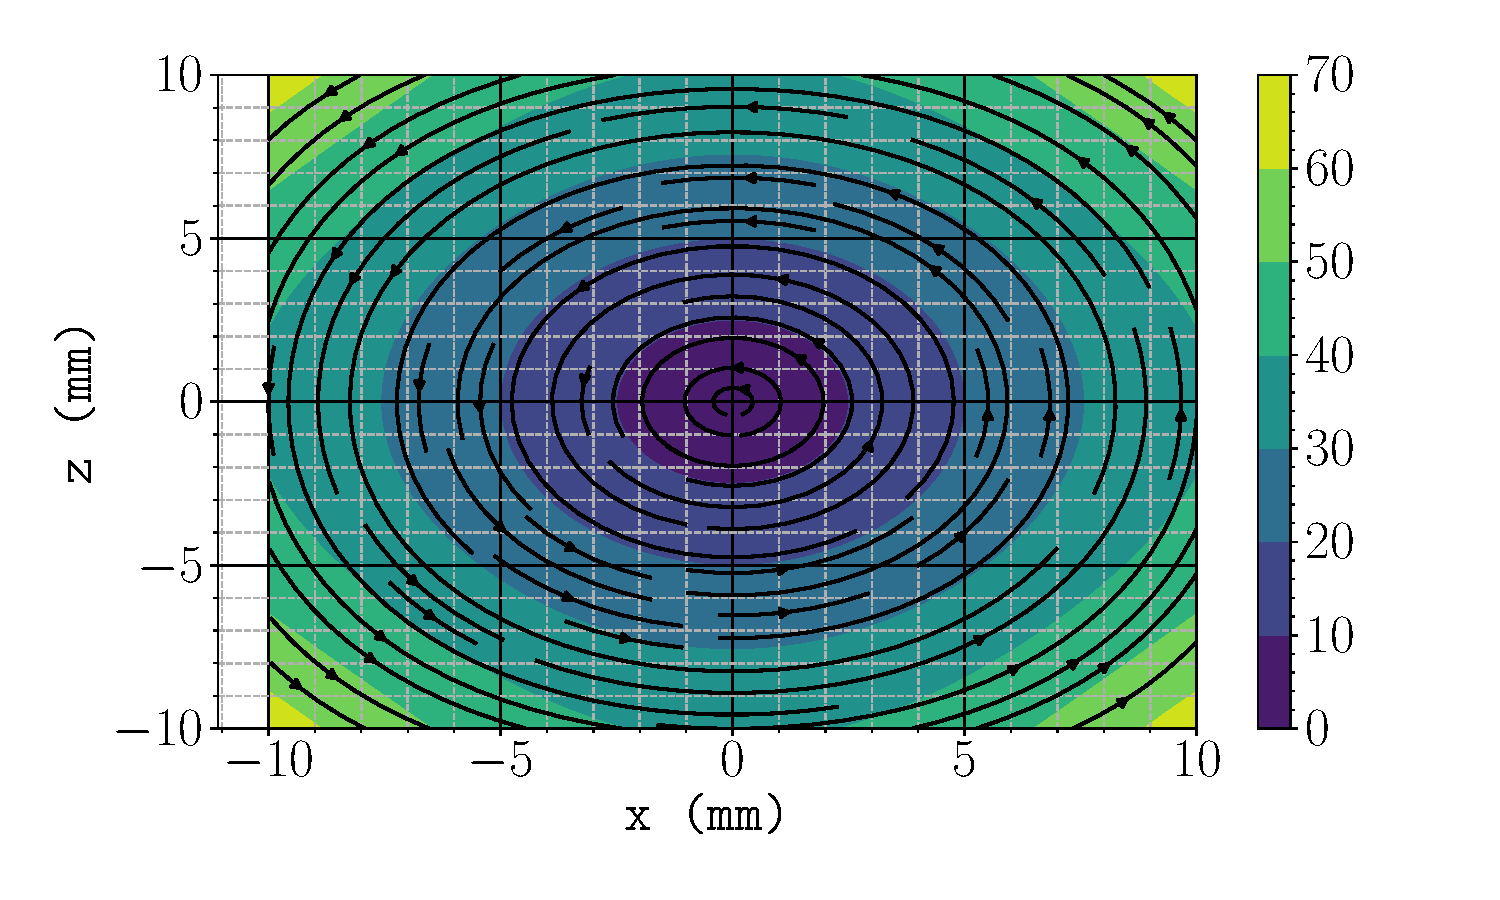
\includegraphics{2D_field_xz.pdf}}\label{fig:2d_field_xz}}
  \subfloat[][]{\scalebox{0.4}{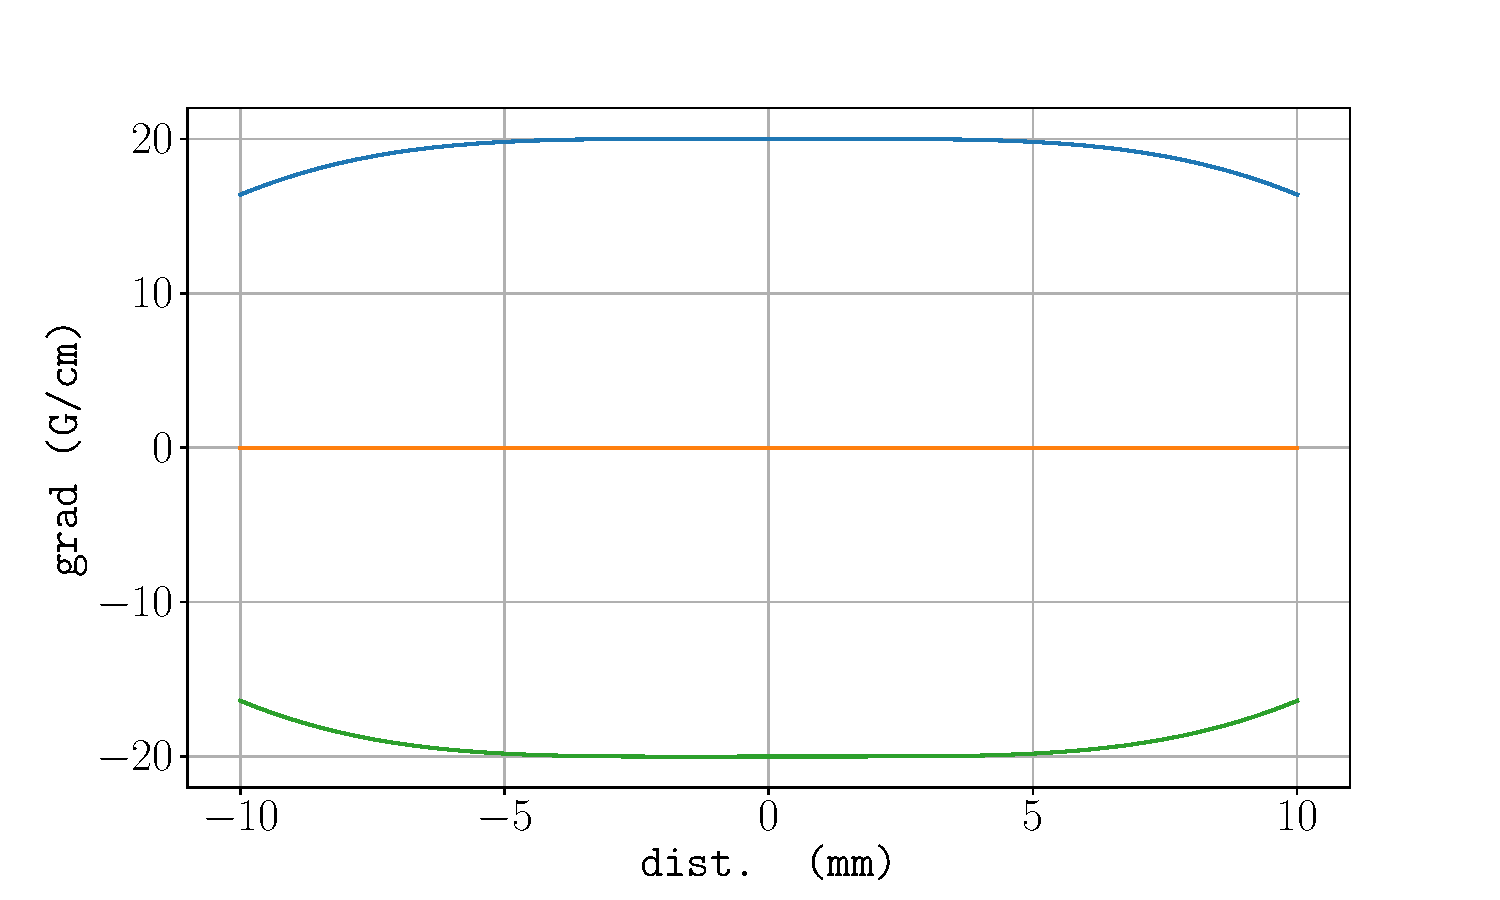
\includegraphics{2D_grad.pdf}}\label{fig:2d_grad}}\\
  \subfloat[][]{\scalebox{0.4}{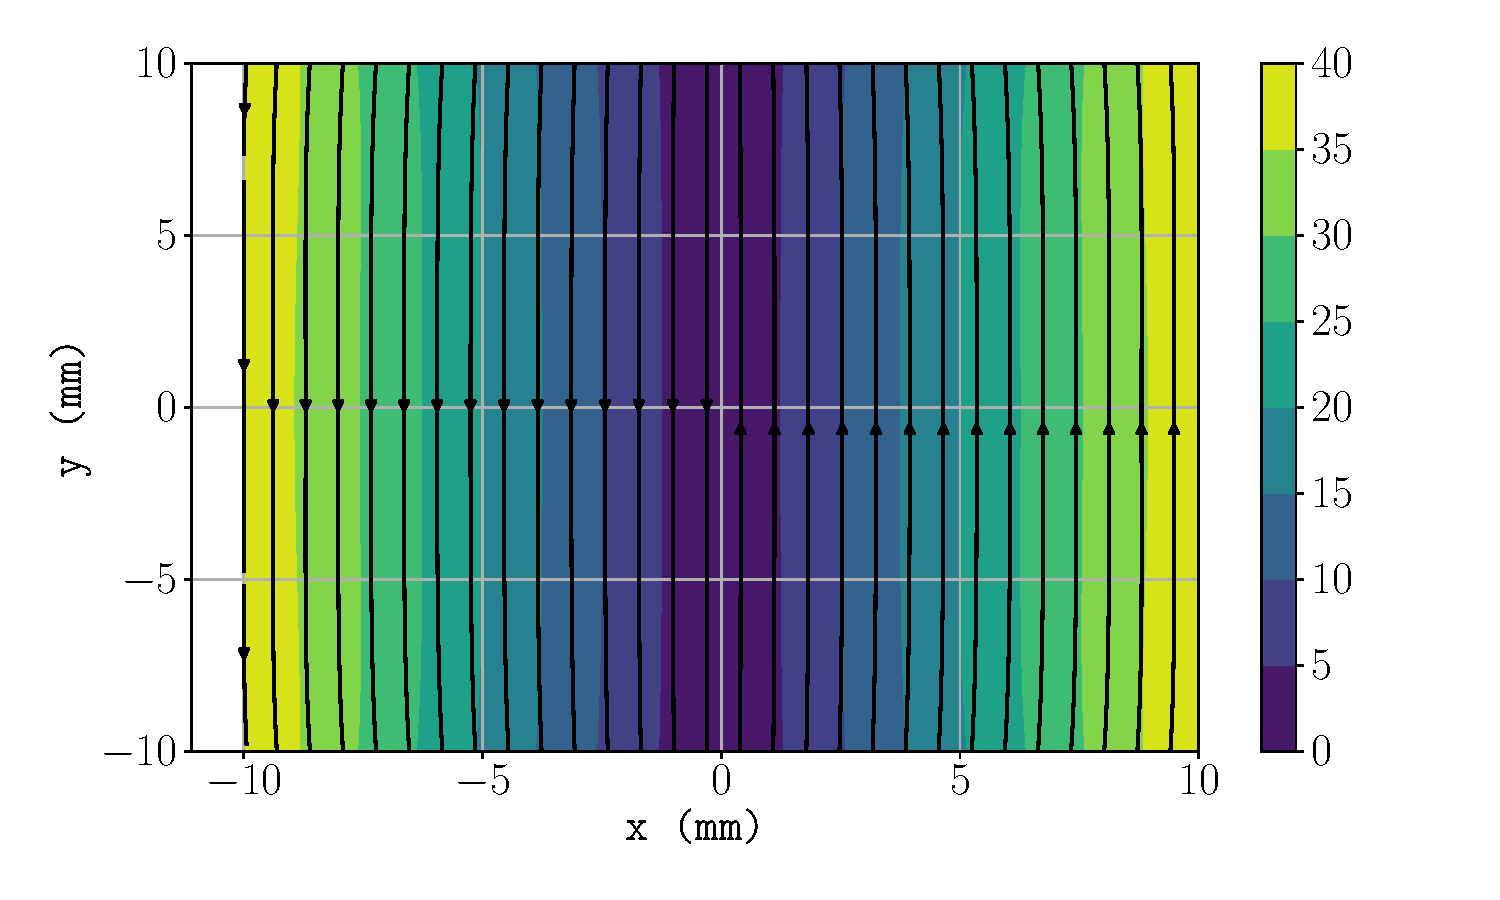
\includegraphics{2D_field_xy.pdf}\label{fig:2d_field_xy}}}
	\caption[Calculated field and field gradients for the 2D \ac{mot} quadrupole
		coils]{Calculated field and field gradients for the 2D \ac{mot}
		quadrupole coils. In this coordinate system, the 2D \ac{mot}cools and
		traps atoms in the \(\vec{x}\) and \(\vec{z}\) directions. The
		simulation was performed using a nominal current of
		\sivalue{1}{\ampere}, which corresponds to a current density in each
		coil of \sivalue{7.78}{\ampere\per\square\milli\metre}. The magnitude of
		the magnetic field (in units of \sivalue{}{\gauss}) and its direction in
		the axial and radial planes of symmetry are shown in \textbf{(a)} and
		\textbf{(b)}, respectively. \textbf{(c)} shows the field gradient
		components \(\partial_x B_x\) (blue), \(\partial_y B_y\) (orange) and
		\(\partial_z B_z\) (green) along their corresponding axes.}
	\label{fig:2d_mot_field_gradient}
\end{figure}
\subsection{The 3D MOT system}\label{sec:3d_mot}
The main chamber contains the apparatus that is used to make a 3D
\ac{mot}~\cite{Raab1987}. Each \ac{mot} beam originates from a \ac{pm} fibre and is collimated using a
lens with a nominal focal length of \sivalue{75}{\milli\metre} to a waist size of \sivalue{7.5}{\milli\metre}. At the output
of each collimator is a \ac{qwp}, with its slow axis oriented at a 45\(^\circ\)
angle to either the fast or slow axis of the fibre, to produce either left- or right-handed circularly polarised light. The \ac{mot} beams along the axial direction of the quadrupole field
(i.e. the \(\vec{z}\) direction) are orthogonally
polarised to the others along the \(\vec{x}\) and \(\vec{y}\) directions. The \ac{mot} beams are aligned so that their intensities at the centre of the chamber are equal, so that the \ac{mot} forms where the magnetic field is zero.
\subsubsection{Spherical quadrupole magnetic field}
The magnetic field for the 3D \ac{mot} is created by a pair of coils in an
anti-Helmholtz configuration. Each coil is wound using rectangular wire coated in a
\sivalue{35}{\micro\metre} thick layer of Pyre-M.L, a UHV-compatible polyamide
which provides a layer of insulation between each loop. The wire has a
cross-section of dimensions \(\sivalue{1.1}{\milli\metre} \times
\sivalue{1.1}{\milli\metre}\), including the insulation. The coils has
20 layers in the axial direction and 12 radially. The
inner diameter of the coil is \sivalue{25.4}{\milli\metre}, to allow for optical
access of the \(\vec{z}\)-axis \ac{mot} beams, and the maximum diameter is
\sivalue{59.2}{\milli\metre} -- small enough that the coil could be
inserted into the chamber through the DN63 CF ports. The coils are mounted to
the chamber using groove grabbers which clamp into grooves inside the wall of
the DN40 ports. The coil formers increase the surface area in contact
with the chamber, increasing the rate of heat dissipation from the
coils. 
\par\noindent 
\FigureRef{fig:mot_coil_temp}~shows the temperature rise of the coils
after they are turned on, both at atmospheric pressure and after evacuating
the chamber. At a low pressure (here around
\sivalue{1e-2}{\milli\bar}), the
temperature of the coils inside the chamber does not exceed
\sivalue{40}{\celsius}. This warms the chamber up by a few degreees,
as shown in~\FigureRef{fig:mot_coil_temp_tg4}. Once mounted, the distance between the
innermost
loops is \sivalue{70}{\milli\metre}. The red and blue circles in~
\FigureRef{fig:coil_a} show the
magnetic field, measured using a Hall probe, along the axis of symmetry for each
of the coils with a current of \sivalue{2.53}{\ampere}.
\FigureRef{fig:coil_b} shows the axial field measured when the coils
are operating together. This shows good agreement with the field
calculated from the Biot-Savart law.
\begin{figure}[!htbp]
	\centering
	\def\svgwidth{\columnwidth}
  \subfloat[][]{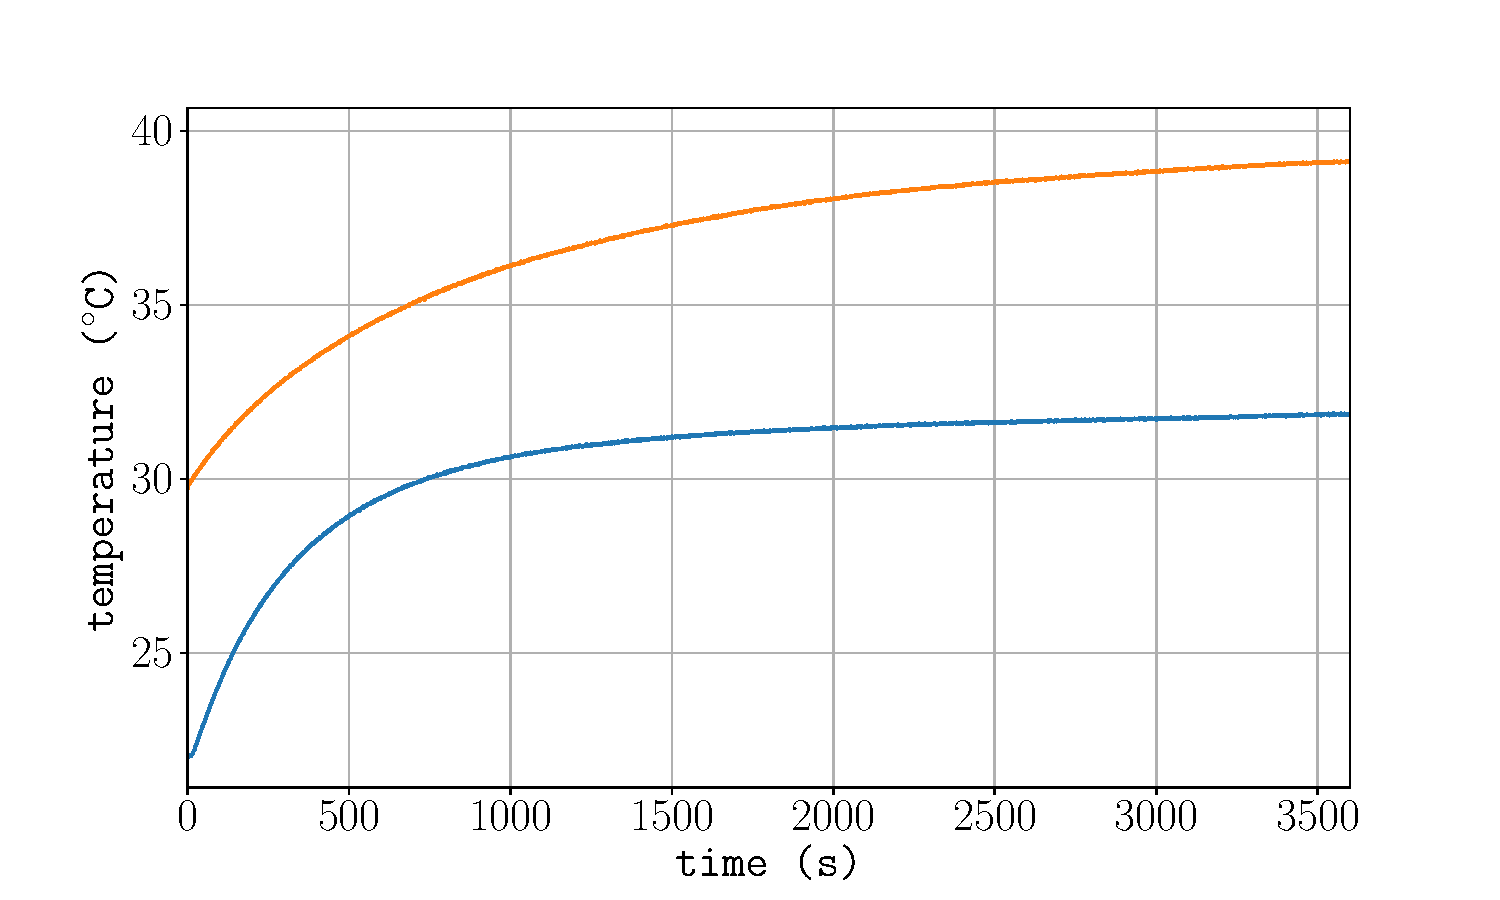
\includegraphics[width=0.45\textwidth]{mot_coil_temperature.pdf}\label{fig:mot_coil_temp}}
	\subfloat[][]{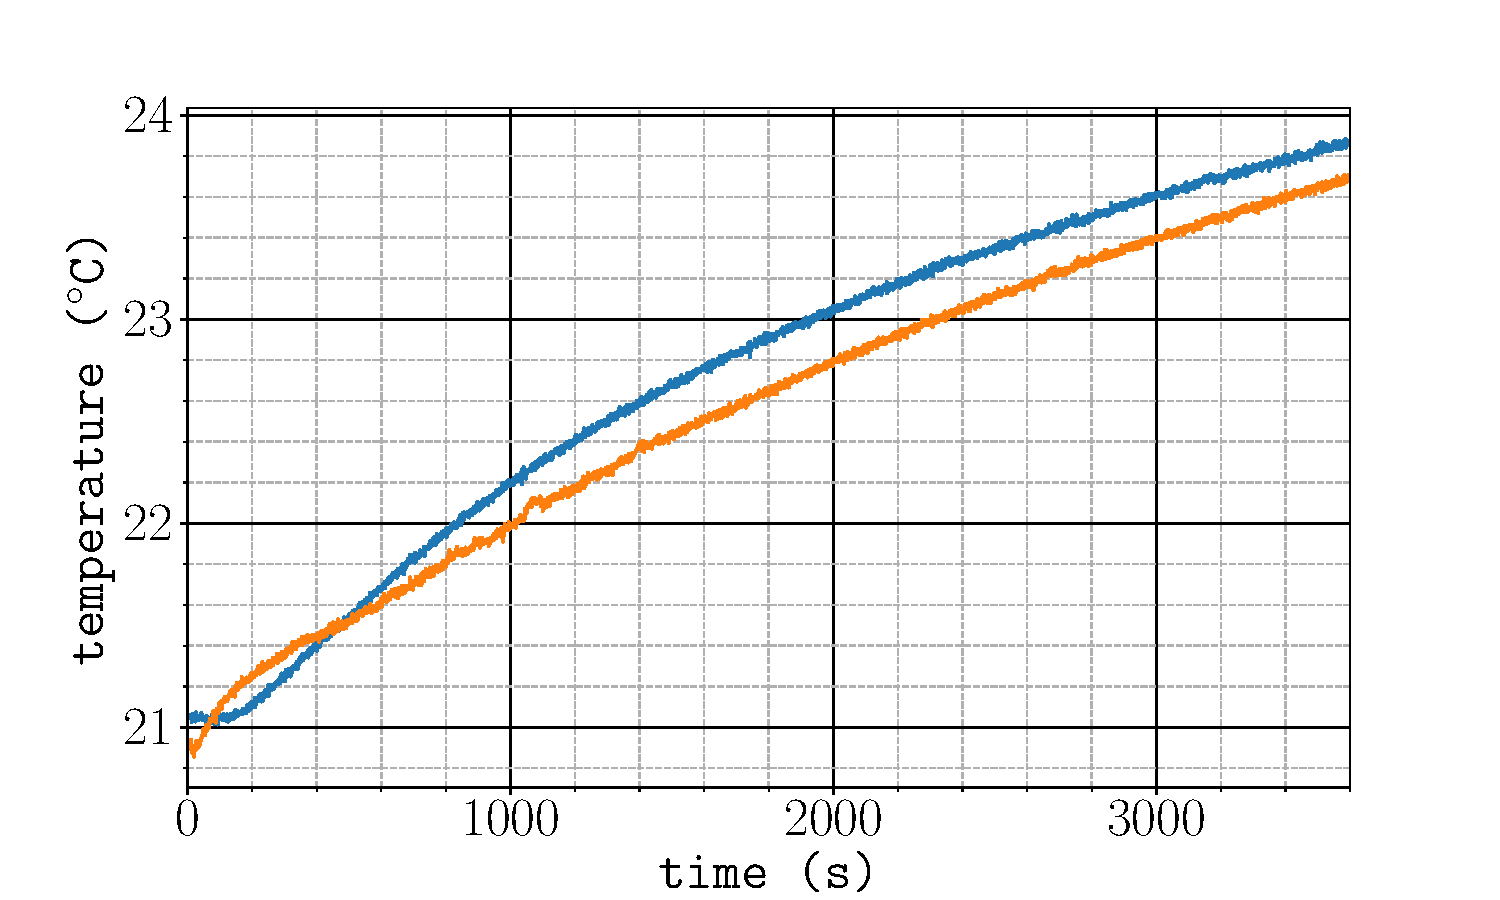
\includegraphics[width=0.45\textwidth]{mot_coil_temperature_chamber.pdf}\label{fig:mot_coil_temp_tg4}}
	\caption[\ac{mot} coil temperature rise]{Temperature rise due to the
  \ac{mot} coils over 1 hour of operation. The blue curves were
measured when the coils were at atmosphere and the orange were
measured under a rough vacuum around \sivalue{1e-2}{\milli\bar}. For
the orange curve, the coils were switched on before $t=0$.
\textbf{(a)} shows the temperature of the coils and \textbf{(b)} is
the temperature of the exterior of the chamber.}
	\label{fig:mot_coil_temp_both}
\end{figure}

\begin{figure}[!htbp]
	\centering
	\def\svgwidth{\columnwidth}
  \subfloat[][]{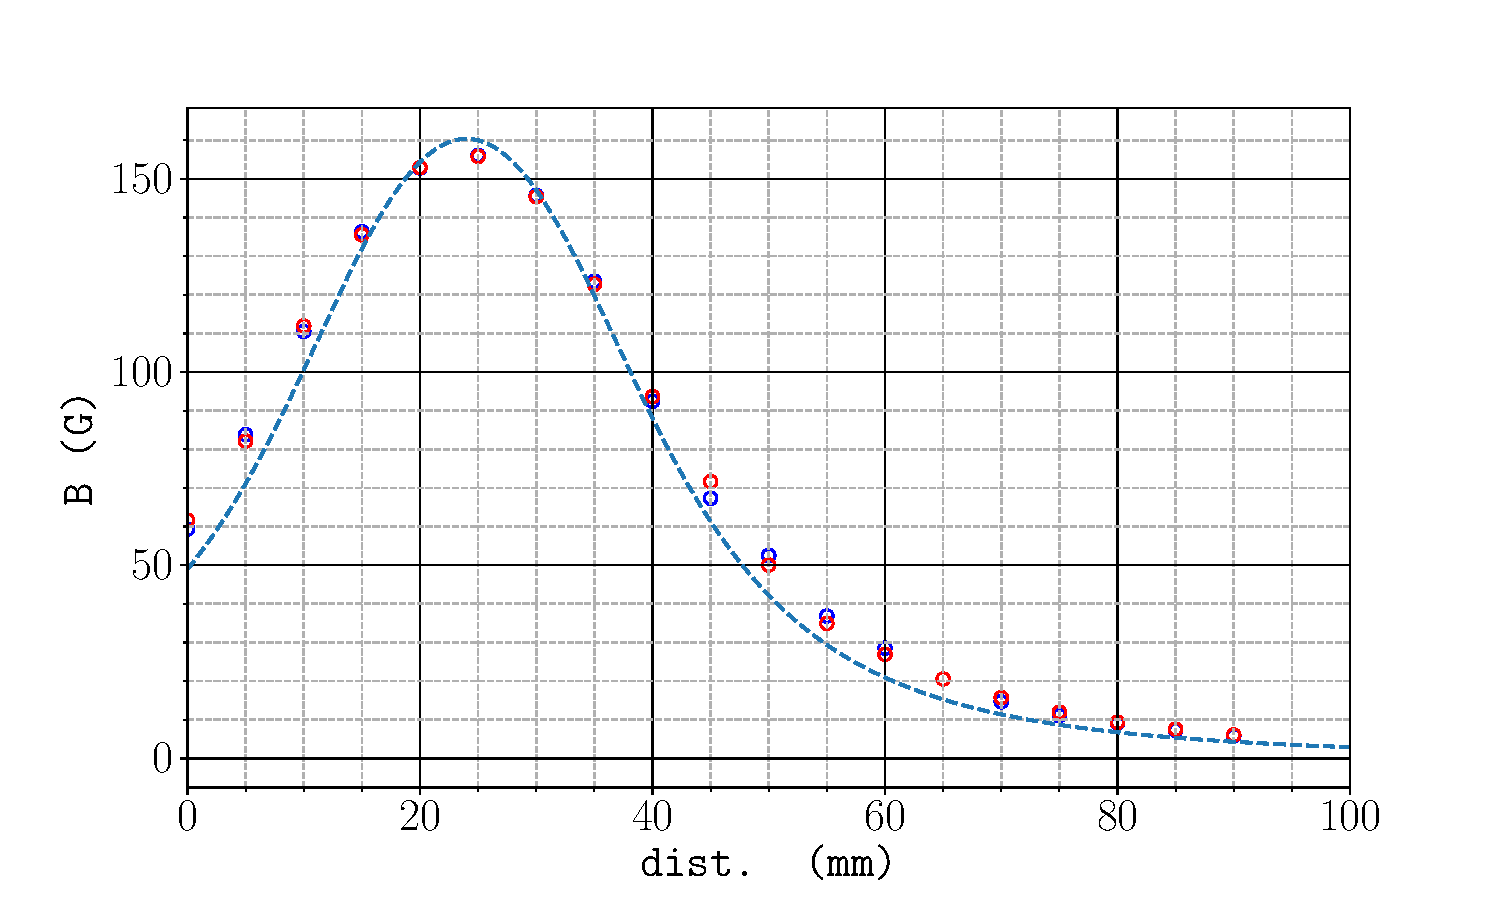
\includegraphics[width=0.45\textwidth]{mot_field_3D.pdf}\label{fig:coil_a}}
  \subfloat[][]{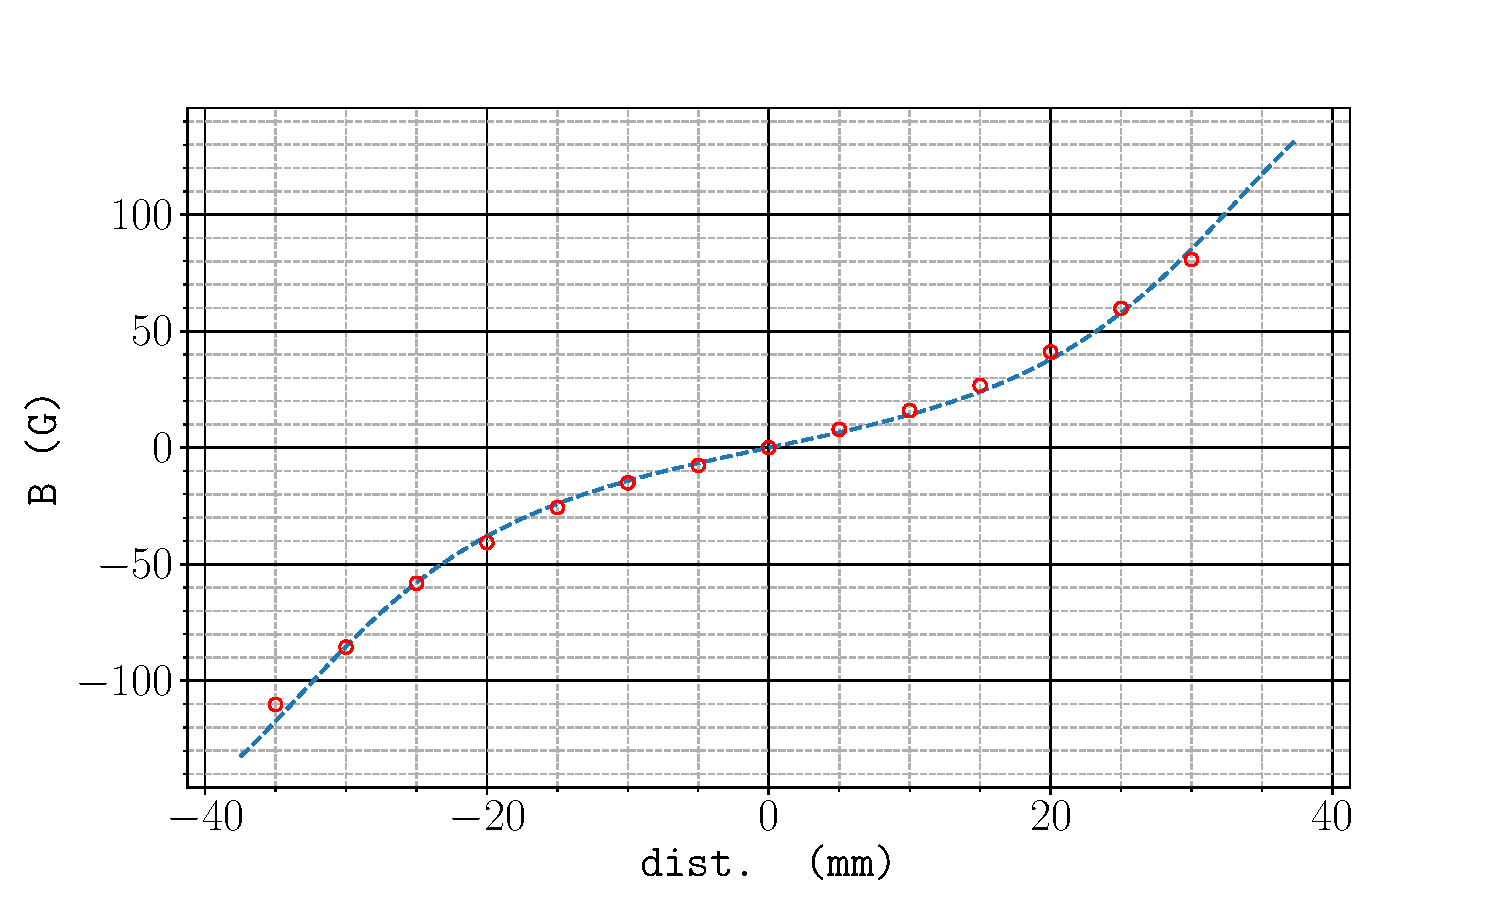
\includegraphics[width=0.45\textwidth]{mot_field_together_3D.pdf}\label{fig:coil_b}}
	\caption[Measured magnetic field and field gradient for the 3D \ac{mot}
		coils]{Measured magnetic field and field gradient for the 3D \ac{mot}
		coils. \textbf{(a)} red and blue circles show the axial magnetic
    field component of both coils as
		measured using a Hall probe.\textbf{(b)} red circles show the
    field close to the centre when the coils are operating together. The dashed lines indicate the axial field as
		calculated from the Biot-Savart law.}
    \label{fig:mot_coil_plots_subfig}	
\end{figure}

%\begin{figure}[!htbp]
%	\centering
%	\def\svgwidth{\columnwidth}
%	\subfloat[][]{\scalebox{0.3}{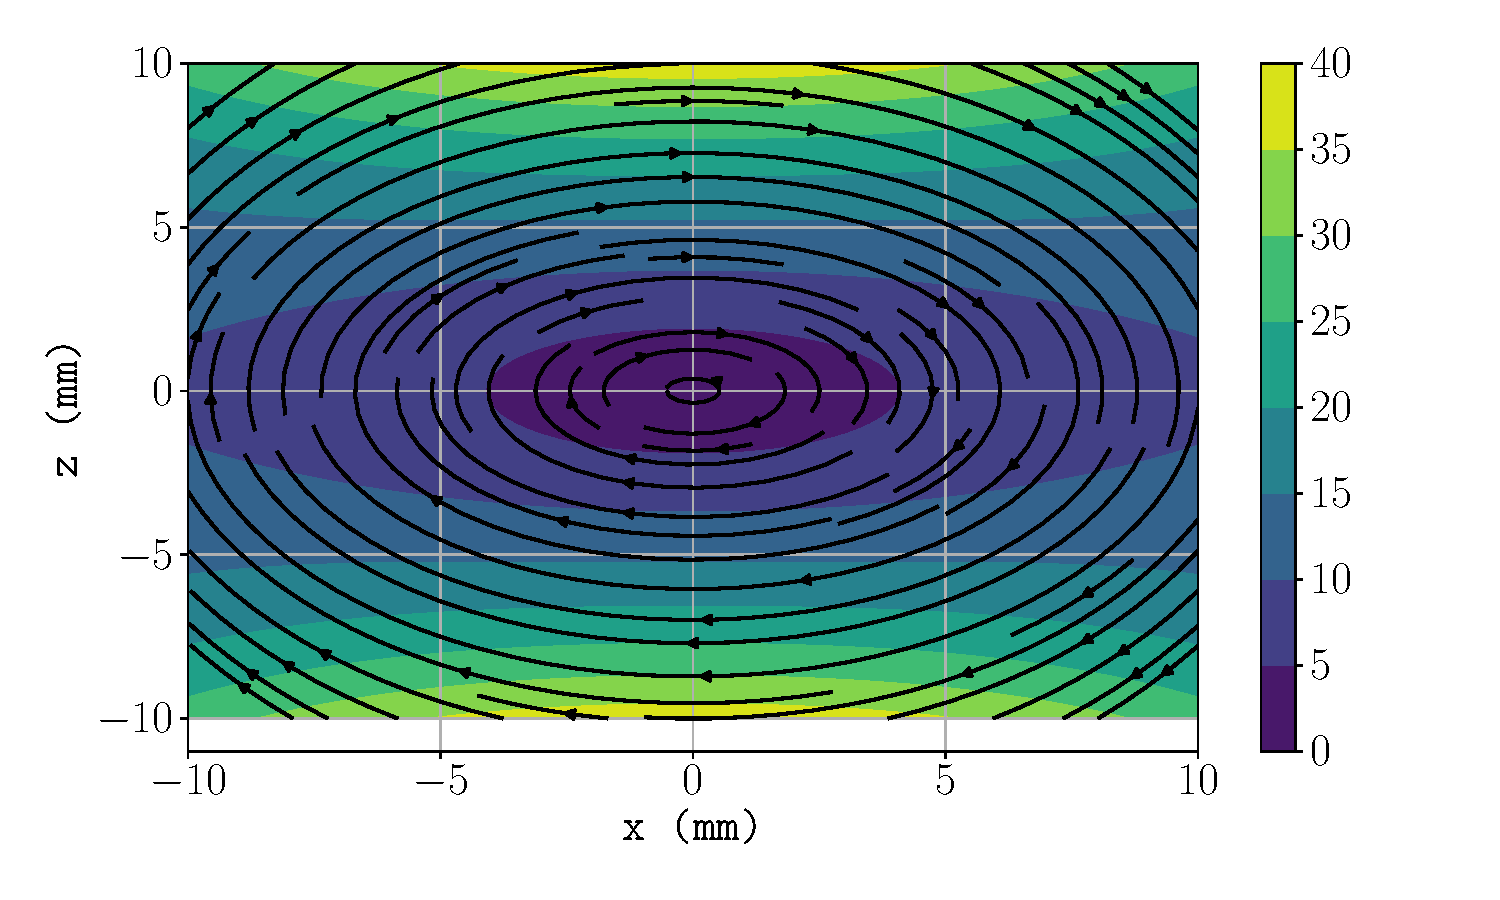
\includegraphics{3D_field_xz.pdf}}\label{fig:3D_mot_axial}}
%	\subfloat[][]{\scalebox{0.3}{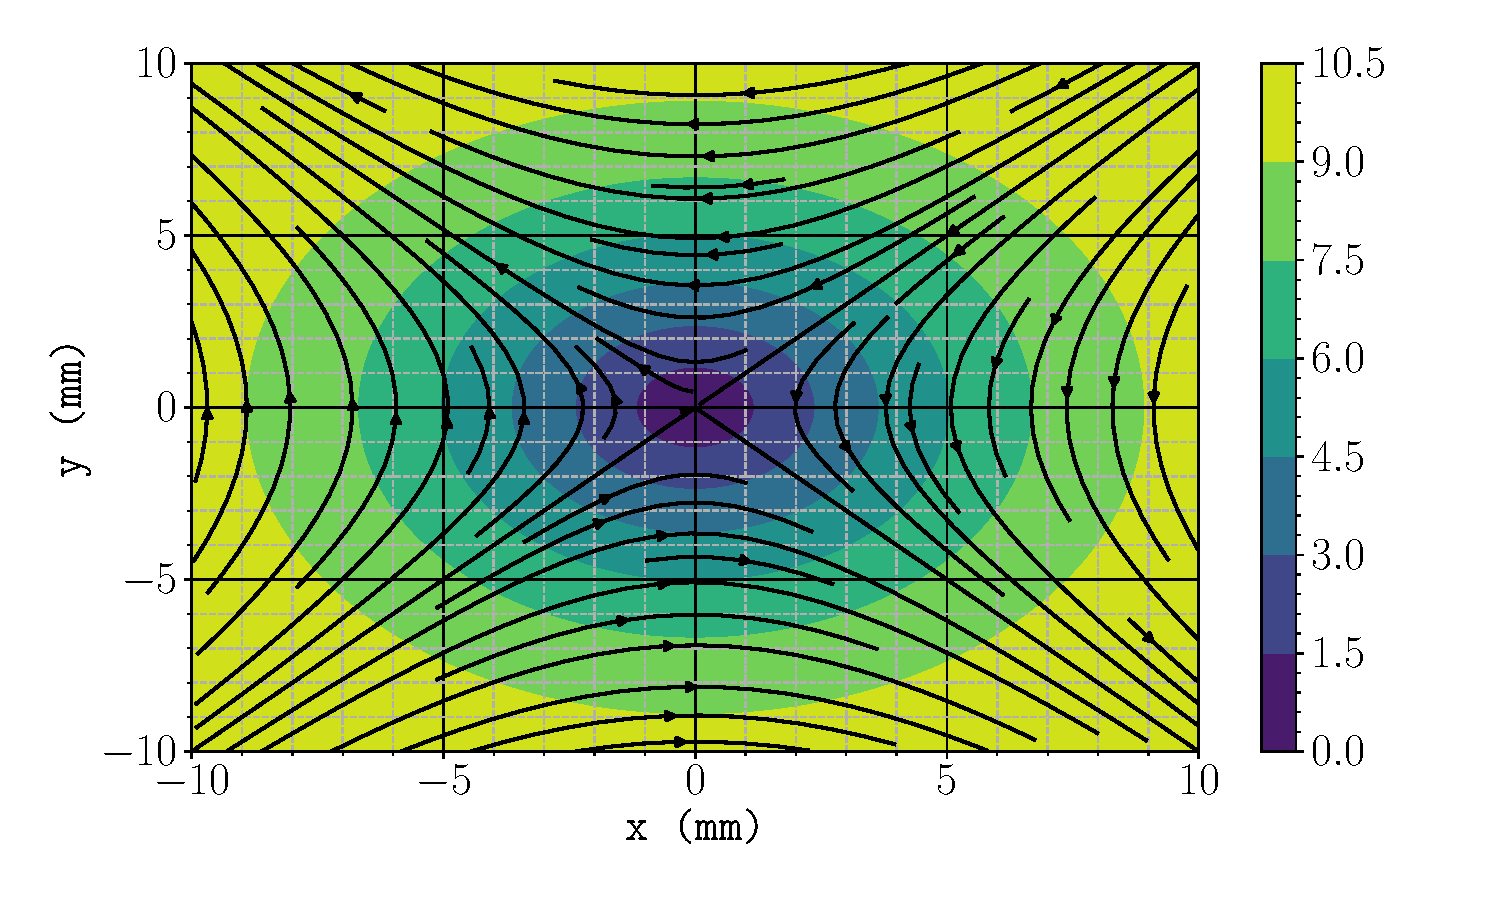
\includegraphics{3D_field_xy.pdf}\label{fig:3D_mot_radial}}}\\
%	\caption[Simulated magnetic field for the 3D \ac{mot} quadrupole
%		coils]{Simulated magnetic field for the 3D \ac{mot} quadrupole coils. In
%		this coordinate system, the axial direction is defined as the
%		\(\vec{z}\) axis. The simulation was performed using a nominal current
%		of \sivalue{2.53}{\ampere}, which corresponds to a current density in
%		each coil of \sivalue{1.33}{\ampere\per\square\milli\metre}. The
%		magnitude of the magnetic field (in units of \sivalue{}{\gauss}) and its
%		direction in the axial and radial planes of symmetry are shown in
%		\textbf{(a)} and
%		\textbf{(b)}, respectively.}
%	\label{fig:3D_mot_field_sim}
%\end{figure}
\subsubsection{Bias Coils}
Three orthogonally arranged pairs of coils are used during the
experiment to provide a homogeneous magnetic field close to the centre of the chamber. In the initial loading and molasses stages, these are used to zero the magnetic field at the centre of the chamber. This is required for effective sub-Doppler cooling. In subsequent stages,
these coils provide a bias field along the appropriate axes during state
preparation, interferometry and state detection. Each coil was wound using
\sivalue{1}{\milli\metre} thick wire and consisted of 5 turns in the
axial direction and 10 turns radially. For a pair of coils in Helmholtz configuration, the magnetic field
gradient at the centre is minimised when the axial separation \(a\) is equal to
the coil radius \(r\), but the geometry of the vacuum chamber meant that it was
not possible to satisfy this condition. The radii and axial separations of each
coil pair are presented in \TableRef{tab:bias_coils}.\begin{table}
	\begin{tabular}{ccccc}
		\toprule
		Axis        & \(a\) (mm) & \(r_i\) (mm) & \(r_o\) (mm) \\
		\midrule
		\(\vec{x}\) & 88         & 105          & 115          \\
		\(\vec{y}\) & 132        & 178          & 188          \\
		\(\vec{z}\) & 116        & 123          & 133          \\
		\bottomrule
	\end{tabular}
	\caption[Table of parameters for each 3D \ac{mot} bias coil.]{Table of
		parameters for each 3D \ac{mot} bias coil. \(a\) denotes the axial
		separation between each coil, measured from their centres. \(r_i\) and \(r_o\) are the inner and
		outer radii, respectively.}
	\label{tab:bias_coils}
\end{table}
\subsection{CCD Imaging}\label{sec:imaging}
During the experiment, atoms are imaged using a CCD camera to spatially resolve the cloud. This was done to measure the temperature using a ballistic expansion method and the trajectory of the cloud (see~\SectionRef{subsec:molasses_imaging}). \FigureRef{fig:imaging_optics} shows a
diagram of the apparatus used for imaging. A pair of \sivalue{125}{\milli\metre}
and \sivalue{50}{\milli\metre} focal length lenses are used to image the cloud
onto a Pike F505-B CCD camera. The camera has a maximum resolution of \(2452 \times
2054\) pixels. A ruler placed in the object plane gave a calibration factor of
\sivalue{7.062\pm 0.048}{pixel\per\milli\metre}. To reduce the level
of background light on the CCD, a bandpass filter is placed in front
of the sensor. This transmits the Rubidium fluorescence at
\sivalue{780}{\nano\metre} with an efficiency of 60\%.
\begin{figure}[!htbp]
	\centering
	\def\svgwidth{0.6\textwidth}
	\input{Figures/Chapter4/ccd_optics.pdf_tex}
	\caption[Optical setup for CCD imaging]{Optical setup for CCD imaging. Two
		lenses are used to magnify the image of the atom cloud on the CCD. A
		bandpass filter is placed in front of the sensor to block out background
		light at wavelengths other than
		\sivalue{780}{\nano\metre}. All lengths are given in millimetres.}
	\label{fig:imaging_optics}
\end{figure}
\subsubsection{Incident Optical Power Calibration} 
Measuring the incident optical power emitted
during resonance fluorescence is useful for estimating the
number of atoms \(N_a\). However, typical number densities in a
\ac{mot} mean that the cloud is optically thick and we see mainly 
the atoms close to the surface. Consequently, the fluorescence can
lead to an under-estimate of the atom number. More accurate techniques such as
absorption imaging can be used, but for the purposes of this
experiment, it was
sufficient to use fluorescence imaging as a rough estimate of the
number of atoms in the \ac{mot}. In subsequent stages of the
experiment, a sensitive photodiode with a high bandwidth was used to
detect the atoms in each hyperfine ground state. Details on this setup
can
be found in~\SectionRef{subsec:photodiode_setup}. \par\noindent
Neglecting absorption, the power incident on the CCD, let us call that
\(P_\textnormal{ccd}\), can be related to the scattering rate per atom
$R_\textnormal{sc}$ as follows
\begin{equation}
	P_\textnormal{ccd} = \frac{\Omega}{4\pi} t R_\textnormal{sc}  \hbar \omega N_a
\end{equation}
where $\Omega/4\pi = $\pow{1.8}{-3} is the fractional solid angle subtended by
the imaging optics, \(t\) is the transmission of the bandpass filter
and 
\(\hbar \omega =
\sivalue{1.6}{\electronvolt}\) is the fluorescence photon energy. For a
two-level system, the scattering rate $R_\textnormal{sc}$ is 
\begin{equation}
  \label{eq:scattering_rate}
  R_\textnormal{sc} = \frac{\Gamma}{2} \frac{s}{1+s+\left(\frac{2
  \delta}{\Gamma}\right)^2}
\end{equation}
where $\Gamma$ is the spontaneous decay rate of the upper level, $\delta$ is
the angular frequency detuning and $s = I/I_\textnormal{sat}$ is the
saturation parameter. This incident power
is then related to the integrated number of pixel counts \(C_\textnormal{int}\)
by
\begin{equation}
	C_\textnormal{int} = \alpha \tau_\textnormal{exp} \eta P_\textnormal{ccd}
\end{equation}
where \(\tau_\textnormal{exp}\) is the exposure time, \(\eta = 0.14\) is the
quantum efficiency of the CCD and \(\alpha\) is a scaling factor that relates
the incident light energy to pixel counts. By varying the
exposure time used to image a collimated beam with a total power of
\sivalue{0.17}{\micro\watt}, the total number of counts recorded by the camera
as a function of exposure time is plotted in~\FigureRef{fig:camera_counts}. This
gives a count scaling factor of \(\alpha\) =
\pow{2.2}{5}\,counts\,\sivalue{}{\per\micro\second\per\micro\watt}.
With this calibration, the number of atoms in the \ac{mot} can be
estimated. This is described further
in~\SectionRef{subsec:loading_rate}.
\begin{figure}[!htbp]
	\centering
	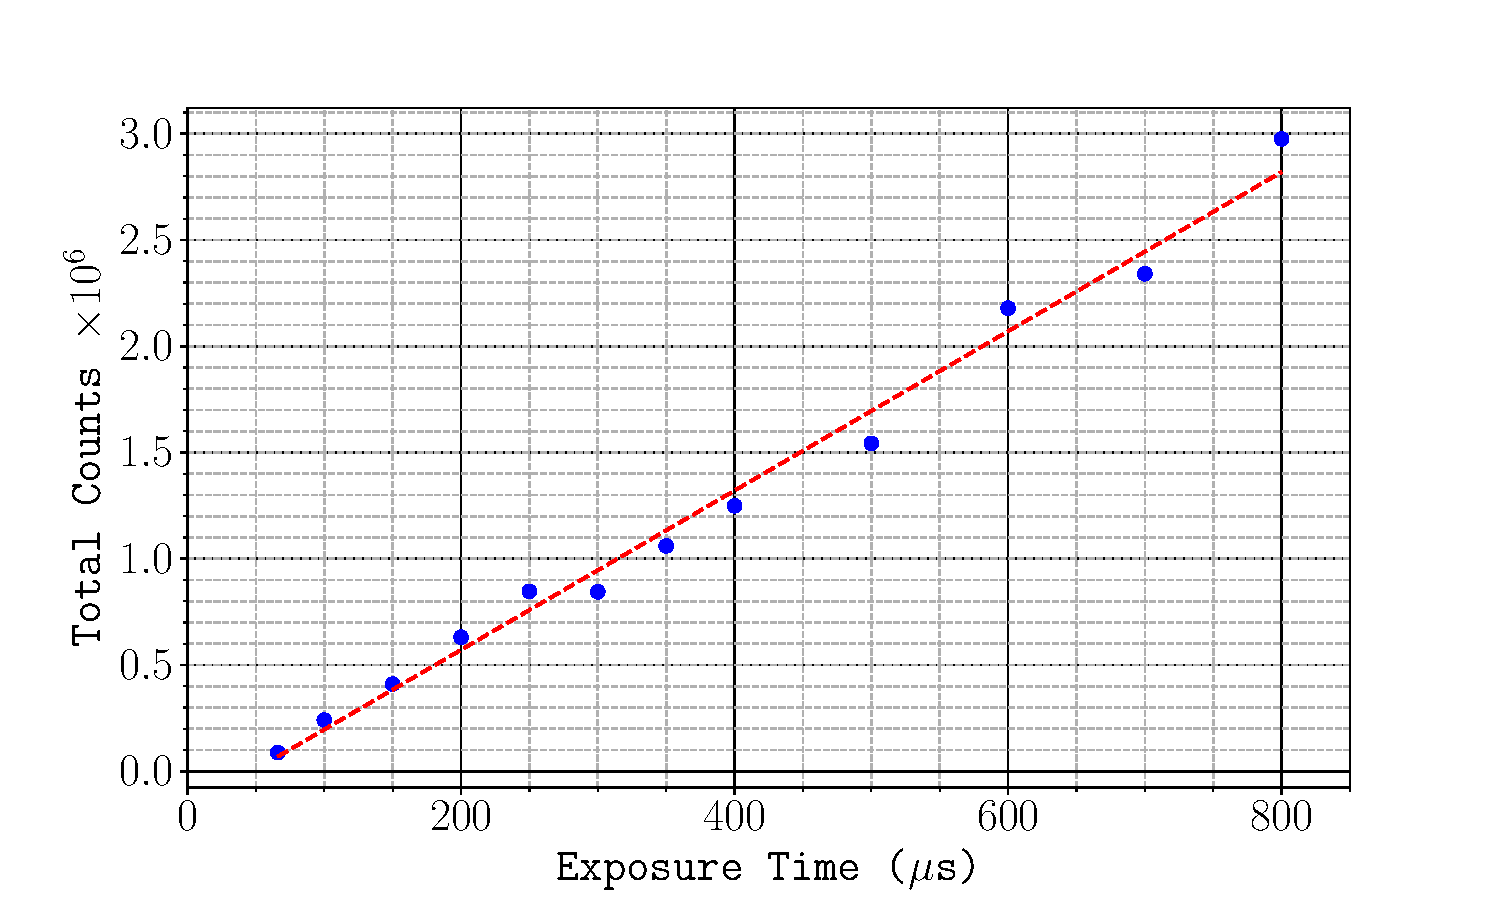
\includegraphics[width=0.5\textwidth]{cam_per_exposure}
	\caption[Integrated pixel counts as a function of CCD exposure
		time.]{Integrated pixel counts as a function of CCD exposure time for an
		incident optical power of \sivalue{0.17}{\micro\watt}. The dashed line
		indicates a linear regression which gives a scaling factor of \(\alpha\)
		=
		\pow{2.2}{5}\,counts\,\sivalue{}{\per\micro\second\per\micro\watt}.}
	\label{fig:camera_counts}
\end{figure}

\section{Generating MOT light}\label{sec:muquans_light}
 All the \ac{mot} light in this experiment was generated by the
 \Muquans\
laser~\cite{muquansWebPage}. \Muquans\ is a French laser company that is a
spin-off from the Institut d'Optique and Observatoire de Paris. A
schematic of
this laser system is shown in \FigureRef{fig:muquans_schematic}. The
light is fibre-coupled to minimise the number of free-space optical components.
This makes the system more stable in the presence of vibrations and
temperature variations. The \Muquans\ laser is comprised of four
\sivalue{1560}{\nano\metre} \acp{ecdl} which are frequency-doubled to produce
light at
\sivalue{780}{\nano\metre}~\cite{Menoret2011}\nocite{Leveque2014}. The first acts as a master laser
which is locked to the \trans{3}{3,4} crossover point in
\ac{rb85} to serve as an absolute frequency reference. The other three slave
lasers are used for output. The first one provides light for cooling \ac{rb87} using the \trans{2}{3} transition.
Light for the \trans{1}{2} repump transition is created by phase modulating this laser using an \ac{eom}.
The other two make up a pair of lasers for driving Raman transitions. One laser
is frequency-offset locked to the master and the other is phase-locked to the
first. This Raman laser was not used in this experiment, so will
not be discussed in further detail. The power in each of these slave lasers is amplified using
an \ac{edfa}. The frequency is doubled to around \sivalue{780}{\nano\metre} using a \ac{ppln}. The output power is controlled using an
\ac{aom}.
\begin{figure}[!htbp]
  \fontsize{8pt}{8pt}
  \resizebox{1\textwidth}{!}{\input{muquans_schematic.pdf_tex}}
	\caption[\Muquans\ Laser System Diagram]{Schematic of the \Muquans\
  laser system. Each output laser is derived from
a\sivalue{1560}{\nano\metre} \acs{ecdl} (shown in green) which is
amplified using an \acs{edfa} and then frequency-doubled to
\sivalue{780}{\nano\metre} using a \acs{ppln} crystal. A master laser
is locked to the 3,4 crossover in \ac{rb85} and the output lasers are
offset-locked to their corresponding frequencies. The dashed region
indicates the components used for generating light for the \acp{mots},
which was the part used for this experiment.}\label{fig:muquans_schematic}
\end{figure}
\subsection{Absolute Frequency Reference}\label{subsec:muquans_master}
The master laser provides an absolute frequency to which the slave
lasers are offset-locked. The reference frequency is created using 
saturated absorption spectroscopy inside a Rubidium vapour cell. The sub-Doppler
features in this spectrum are insensitive to temperature changes, and 
have linewidths close to the natural linewidth of
Rubidium (\(\Gamma \sim 2\pi \times 6\) MHz). \FigureRef{fig:muquans_satspec}
shows the saturated absorption spectrum using the \Muquans\ master laser. The frequency is varied
by finely adjusting the temperature of the master \ac{ecdl}. The
master laser is set to lock to the crossover resonance between the \(F = 3
\rightarrow F' = 3\) and \(F = 3 \rightarrow F' = 4 \) transitions in \ac{rb85}
(indicated as \textbf{(b)}), which is the strongest feature in the
spectrum. This crossover is around \sivalue{1.1}{\giga\hertz} above the cooling
transition in \ac{rb87} (indicated as \textbf{(a)}).
\begin{figure}[!htbp]
	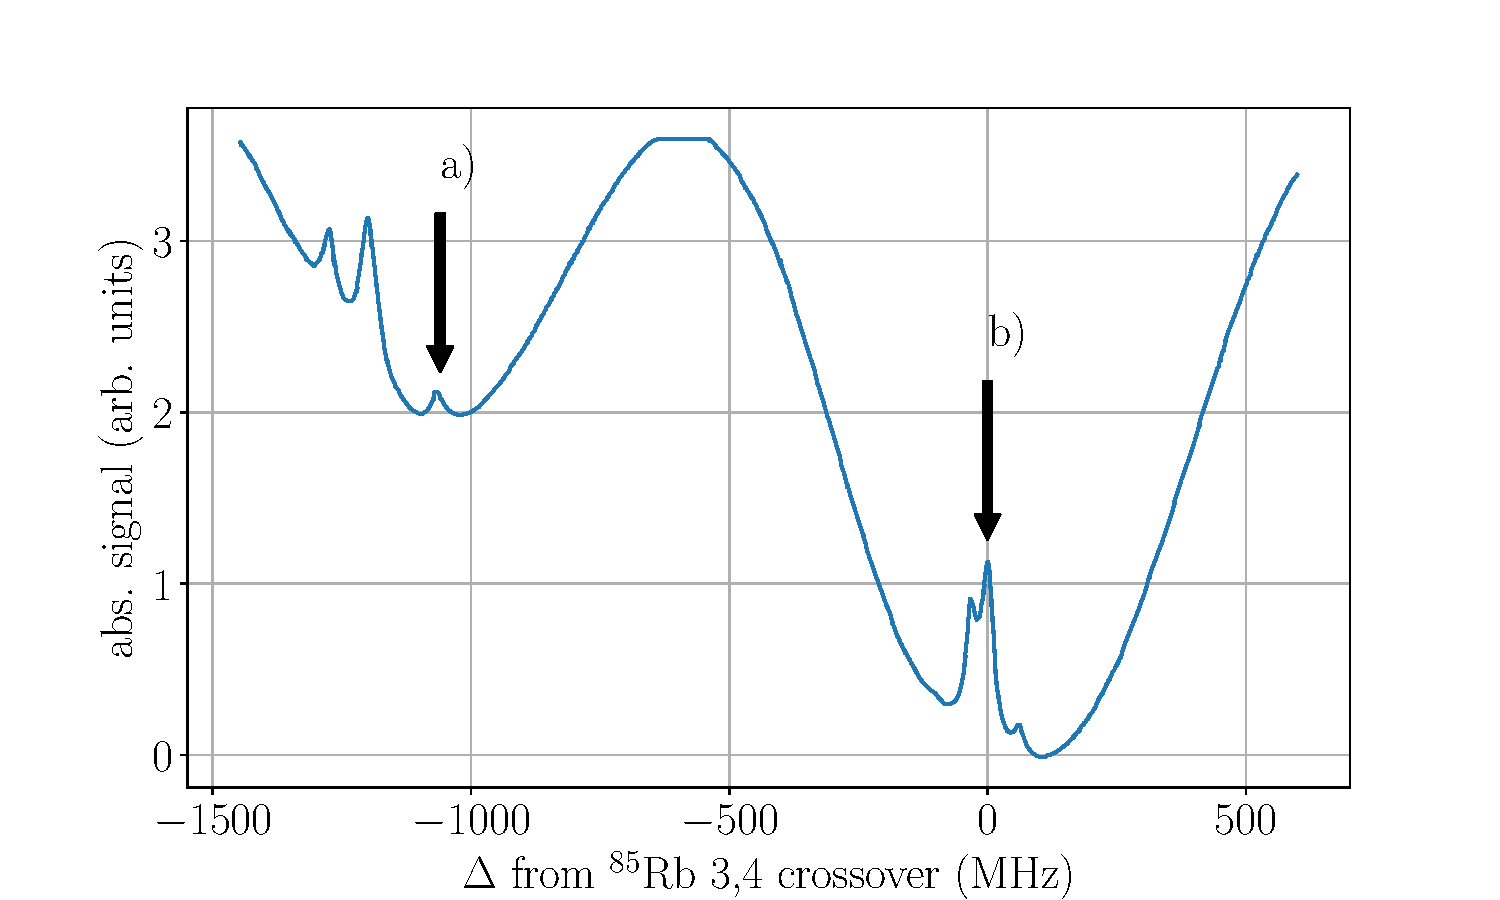
\includegraphics[width=0.6\textwidth]{sat_spec}
	\caption[Saturated absorption spectroscopy of the \\Muquans\ master laser.]{Saturated absorption spectroscopy using the Rubidium vapour cell in the \Muquans\ laser. The absorption features indicated are \(a\): the \(F = 2 \rightarrow F' = 3\) transition in \ac{rb87} and \(b\): the crossover resonance between the \(F = 3 \rightarrow F' = 3\) and \(F = 3 \rightarrow F' = 4 \) transitions in \ac{rb85} which is used to lock the frequency of the master laser.}\label{fig:muquans_satspec}
\end{figure}
\begin{figure}[!htbp]
	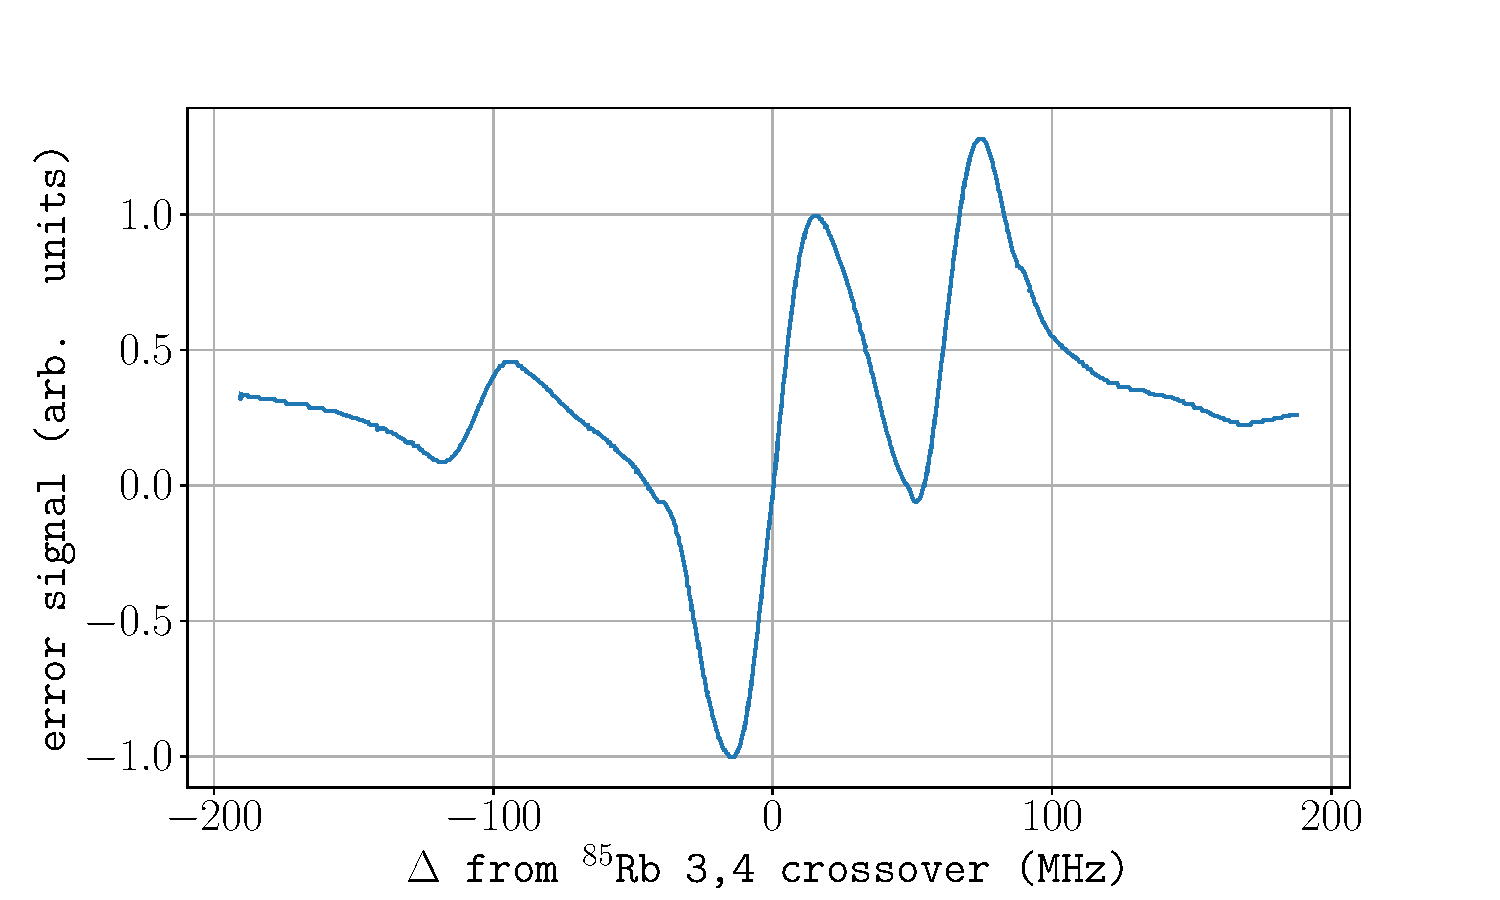
\includegraphics[width=0.6\textwidth]{error_signal}
	\caption[Error Signal for the \Muquans\ master servo.]{Error signal obtained by modulating the laser current. Close to the lock point, the signal is approximately linear. This signal is used in a feed-back loop to correct for frequency changes of the master laser.}\label{fig:muquans_error_signal}
\end{figure}
The frequency of the laser is dithered by modulating the current to
the \ac{ecdl}~\cite{Supplee1994}. Phase-sensitive detection using a
lock-in amplifier then produces the derivative signal shown in
\FigureRef{fig:muquans_error_signal}. Close to the lock point that
provides an error signal that is
proportional to the frequency difference from the lock point. The servo that controls the master laser frequency also contains
an integrator to compensate for long-term drifts arising from temperature
variations.
\subsection{Cooling and Repump Light}
The first of the slave lasers provides light to address the cooling
transition. This is
frequency-offset locked to the master by comparing their beat frequency to a
reference from a \ac{dds} (labelled as $f_0$
in~\FigureRef{fig:muquans_schematic}). The reference is multiplied by a factor
of 8 before it is mixed with the beat frequency of the
\sivalue{1560}{\nm} light. After frequency doubling and taking into account the frequency shift of
the output \ac{aom} and those used to control each \ac{mot} beam
(see~\SectionRef{sec:mot_control}), a \ac{dds} frequency of
\sivalue{88.82}{\MHz} offsets the frequency of the slave laser from
the master laser's frequency so that it is resonant with the
\trans{2}{3} cooling transition. Similarly, a \ac{dds} frequency of
\sivalue{87.89}{\MHz} red-detunes the slave laser from this transition
by \sivalue{15}{\MHz}. A plot of the error signal used to lock this offset
frequency is shown in \FigureRef{fig:slave_offset}. The zero-crossing
occurs when the frequency difference of the two lasers is equal to
$8 f_0$. 
\begin{figure}[!htbp]
	\centering
	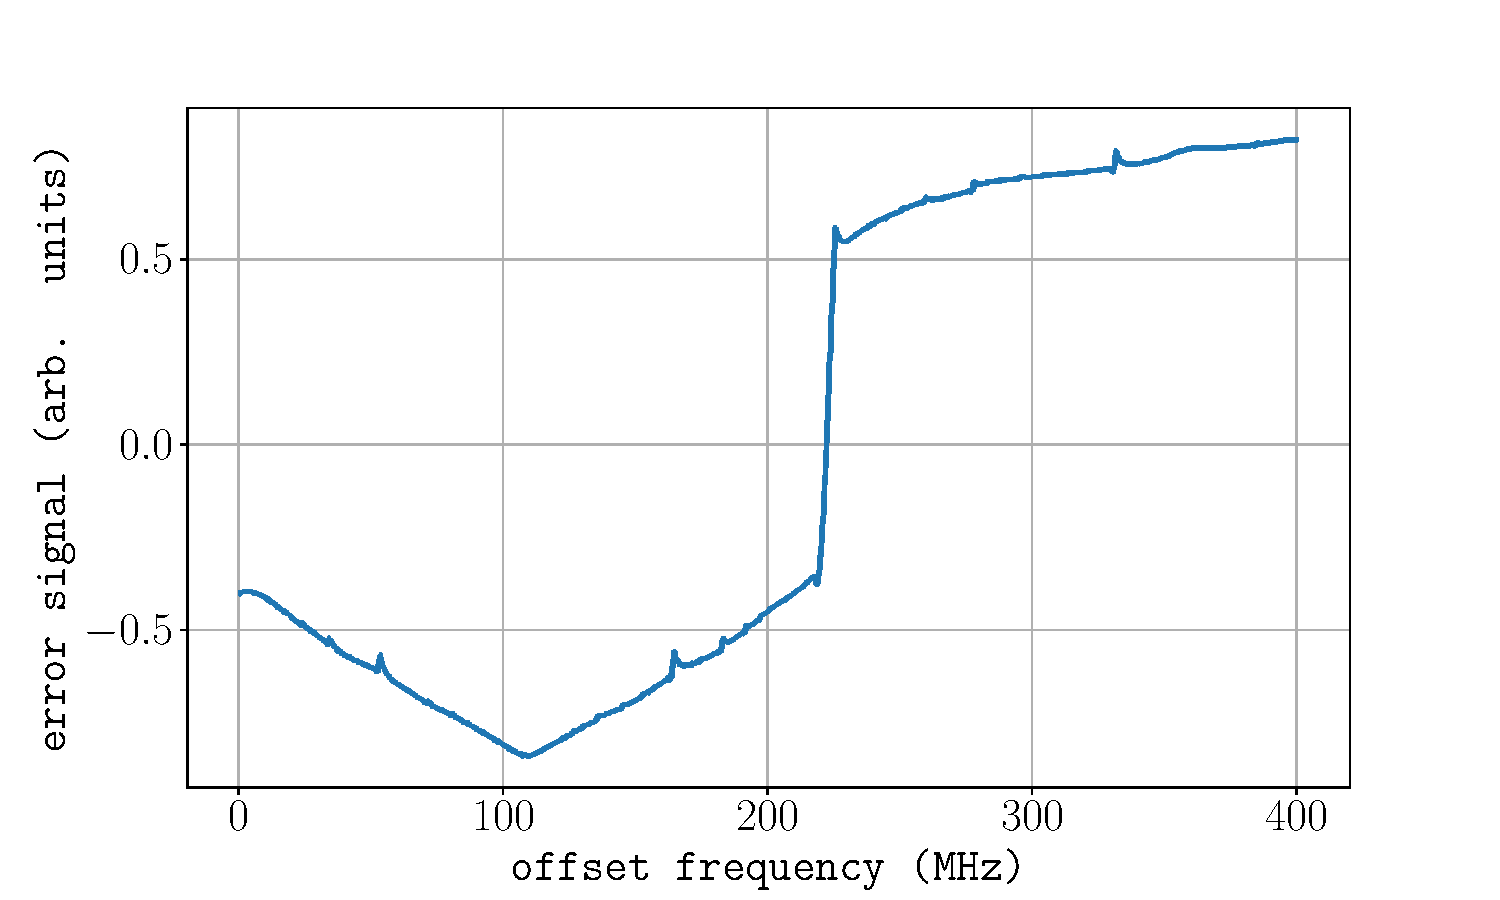
\includegraphics[width=0.6\textwidth]{slave0_error}
	\caption[Error Signal for the \Muquans\ Cooling laser.]{Error signal
  for the \Muquans cooling laser, plotted as a difference from the
reference frequency. The beat frequency between the master and slave
lasers is compared to a reference frequency generated by a \ac{dds}
(see text). A servo loop feeds-back onto the frequency of the slave laser to keep this difference close to zero.}\label{fig:slave_offset}
\end{figure}
\par\noindent 
An \ac{eom} modulates the phase of the cooling laser to
produce light for the \trans{1}{2} repump transition. This modulation
creates frequency sidebands separated by integer multiples of the
modulation frequency. If the amplitude of the modulation is small, only the first
positive and negative sidebands are present. When the carrier is set
to drive the cooling transition, the modulation frequency is set so that the first
positive sideband drives the repump transition, which is
\sivalue{6.6}{\GHz} higher in frequency. A separate \ac{dds} provides
the reference for the modulation frequency (labelled as $f_m$
in~\FigureRef{fig:muquans_schematic}), so that the frequency of
the cooling and repump
light can be independently ramped during the experiment (see
\SectionRef{subsec:muquans_comm}). The \ac{dds} frequency is amplified, doubled and subtracted
from a \sivalue{3.5}{\giga\hertz} reference signal to give the
modulation frequency for the \ac{eom}. A \ac{dds} frequency of $f_m
=$\sivalue{104.25}{\MHz} produces a positive sideband to drive the
\trans{1}{2} transition when the carrier is \sivalue{-15}{\MHz} below
the \trans{2}{3} transition. The modulation power is externally controlled using a \ac{vca} to control the ratio of
repump power to cooling power. An RF switch turns the repump on and off by blocking the reference frequency. 
\par\noindent 
The total output power is controlled using an
\ac{aom} that has a fixed modulation frequency of
\sivalue{110}{\mega\hertz}. \FigureRef{fig:muquans_cooling} shows
the combined power of the cooling light for the 3D \ac{mot} as a
function of the control voltage to the \ac{aom}
RF power. The hardware used to divide the light from the laser to the
separate beams is described in~\SectionRef{subsec:optical_fibre}.
\begin{figure}[htpb]
  \centering
  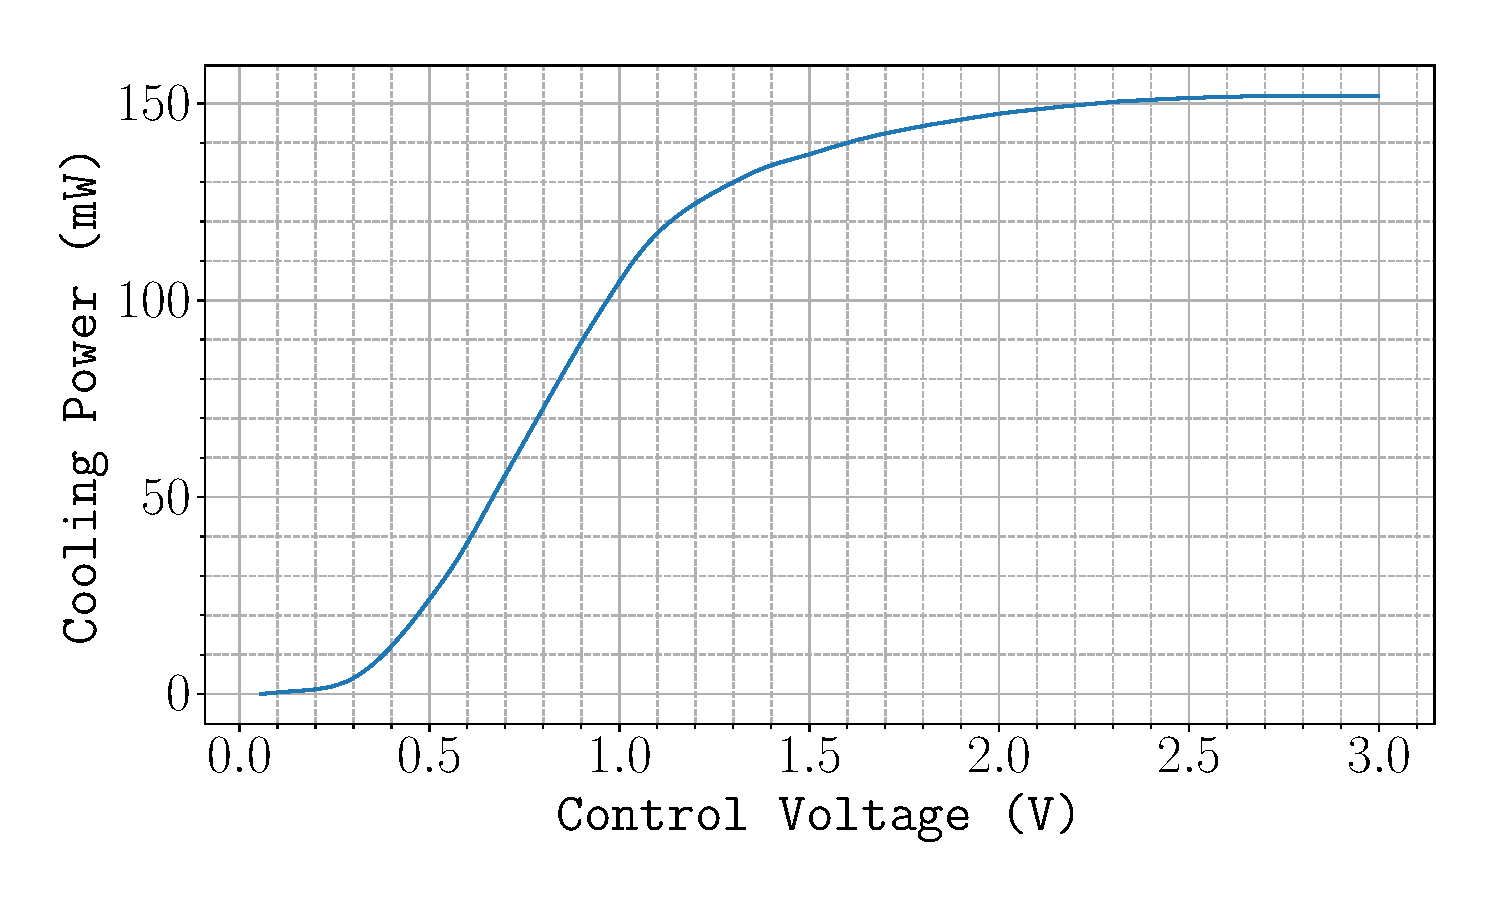
\includegraphics[width=0.8\linewidth]{muquans_cooling.pdf}
  \caption[Cooling power vs. \ac{aom} control voltage.]{Combined
  3D \ac{mot} cooling power as a function of control voltage for the
  RF power that drives the
\Muquans output \ac{aom}.}
  \label{fig:muquans_cooling}
\end{figure}
\subsection{Real-Time Control} \label{subsec:muquans_comm}
During the experiment, it is necessary to vary the frequency and power
of both
the cooling and repump light.
Analogue and digital signals control the RF sources for the output
\ac{aom} and
\ac{eom}. A \ac{dds} generates each RF frequency, so that they can be
updated in real-time.
These are also
programmed to ramp the output frequency for a specified duration and
ramp rate. This is done by sending serial messages to an
application which interprets the message and synchronously communicates the command to the \ac{dds} using
\ac{spi}. A glossary of the messages and their function is given
in~\AppendixRef{app:serial_commands}. The command is stored in memory
on-board the \ac{dds} and
is triggered to start using a digital pulse. This means that the time at
which the frequency of the light changes is synchronised with the rest
of the experiment. 
\section{Controlling the MOTs}\label{sec:mot_control} Effective
trapping and cooling of Rubidium requires careful control of the light
and magnetic fields used to create the \ac{mot}. A well-balanced
\ac{mot} requires circularly polarised beams with equal intensities so
that there is no net force from scattering light. Otherwise, the
\ac{mot} forms at a position where the magnetic field is not
zero~\cite{Steane1992}. Equivalently, the \ac{mot} requires good
control of the magnetic field inside the chamber. What follows is a
description of the hardware used to implement this control.
\SectionRef{subsec:optical_fibre} describes the network of optical
fibres used to control the frequency and power in each \ac{mot} beam.
The electrical circuits used to control the strength of each bias
field, as well as switching off the quadrupole coils, are described
in~\SectionRef{subsec:coil_control} 
\subsection{Optical Fibre
Network}\label{subsec:optical_fibre} A network of fibre-based
beam-splitters and \acp{aom} distributes the light from the \Muquans
fibre to each of the beams for the 2D and 3D \acp{mot}. This provides
independent control of the power and frequency of the light at each
output of the fibre network. A diagram of this setup is shown
in~\FigureRef{fig:fibre_network}. The \Muquans fibre output is
polarised using a polarising beam-splitter before a \ac{hwp} aligns it
with the slow axis of a \ac{pm} fibre. The light is first divided on a
1:2 beam-splitter, with 66\% exiting one port, used for the 3D
\ac{mot}. The 34\% on the other port is split again using a 95:5
beam-splitter in the hope of making 32\% of the input power available
for the 2D \ac{mot}, leaving 1.7\% for the push beam.
The junctions between components are spliced together to minimise
insertion loss, but still the output powers are significantly lower than that, as
indicated in~\FigureRef{fig:fibre_network}. The slow axes of the spliced fibres are aligned so that the
linear polarisation of the light is maintained. Independent control of each
output is done using a \textit{Gooch and Housego} fibre \ac{aom} with
a central modulation frequency of \sivalue{135}{\mega\hertz}. \par\noindent The light
for the 3D \ac{mot} is split using a 1:3 splitter into pairs of
outputs for the light along the \(\vec{x},\vec{y}\) and \(\vec{z}\)
axes. Unlike the outputs for the $\vec{x}$ and $\vec{y}$ axes, the two used for light
along the \(\vec{z}\) axis have separate \acp{aom}. This is done so
that during the experiment, a single beam along the \(\vec{z}\) axis
can used to blow away background atoms (see
\SectionRef{subsec:blow_away} for more details).

\begin{figure}[!htbp] 
  \centering 
  \fontsize{18pt}{18pt}
  \resizebox{0.5\textwidth}{!}{\input{Figures/Chapter4/fibre_network.pdf_tex}}
  \caption[Network of optical fibre splitters and \acp{aom} for
  \ac{mot}light distribution]{Fibre splitter and \acp{aom} for
  \ac{mot} light distribution. The polarisation of the cooling and
repump light from the \Muquans laser is aligned to the fibre network
using a \ac{pbs} and \ac{hwp}. Apart from the outputs for the
\(\vec{x}\) and \(\vec{y}\) 3D \ac{mot} beams, which have a single
\ac{aom} per axis, the power and frequency at each output can be
controlled independently. The percentages shown are the relative power
at each output, accounting for insertion loss and driving each
\ac{aom} with the optimum RF power.} 
\label{fig:fibre_network}
\end{figure} 
\subsection{Magnetic Field Control}\label{subsec:coil_control} 
There are 5 pairs of bias coils used to control the zero of magnetic
field - 3 for the 3D \ac{mot} and 2 for the 2D \ac{mot}. 
%The radial position of the magnetic field zero can then be
%controlled using bias coils along the other two axes, so that the
%2D \ac{mot} forms along the axis which is co-linear with the central
%axis of the pinhole. In contrast, 3 pairs of coils are used for the 3D
%\ac{mot} so that the position of zero magnetic field coincides
%with the position where the scattering rate from each beam is the
%same. \par\noindent
The current through each set of
bias coils is
controlled using a voltage-controlled current source. The control
voltage is an input at the non-inverting terminal of an OPA549 op-amp.
The coils are placed in series with a sense resistor of resistance
\(R_s\) at the output. The circuit is configured so that the voltage
at the inverting terminal is \(V_- = i R_s\).  This forms a negative
feed-back loop to keep the output current constant if the load
resistance changes. The bias coils can be supplied with up to
\sivalue{2}{\ampere} using a control voltage of \sivalue{10}{\volt}. This same circuit is used to control the 3D \ac{mot}
coils.
\par \noindent
During the experiment, the 3D \ac{mot} coils need to be
switched off rapidly, to allow for effective sub-Doppler cooling of
the atoms~\cite{Dedman2001}. By actively controlling the current
through the coils, their stored energy can be dissipated faster than
the natural time constant \(\tau = L/R\). This is done by applying a
negative voltage across the coils. A flux-gate magnetometer
was used to measure the time taken to switch off the coils. With an
applied voltage of \sivalue{0}{\volt}, the characteristic decay time
is \(\tau = \) \sivalue{2.5}{\milli\second}. Under the maximum
available backward bias of \sivalue{-24}{\volt}, the field can be
completely switched off in \sivalue{800}{\micro\second}. \par\noindent
The quadrupole coils for the 2D \ac{mot} are switched off in much the
same way. An IGBT cuts the flow of current when the gate voltage drops
below a threshold value. To prevent damage to the transistor, a diode
and \sivalue{10}{\ohm} power resistor are placed in parallel with the
coils. This allows the current generated by the back-EMF to dissipate
without damaging the IGBT. These field from these coils can be
switched off in less than \sivalue{1}{\milli\second}.

\section{Characterising the MOTs}\label{sec:mot_characterisation}
This section discusses the performance of the 2D and 3D \acp{mots} for trapping
and cooling \ac{rb87}. The main goal of this stage of the experiment is to
quickly produce an ensemble of trapped, cold atoms in the 3D \ac{mot}. For this
reason, the loading rate of the 3D \ac{mot} is a useful figure-of-merit. As
further cooling in an optical molasses is necessary to achieve a sufficiently
cold ensemble for interferometry (see \SectionRef{sec:optical_molasses}), the
temperature of atoms in the \ac{mot} will not be discussed in detail.
\par\noindent \nocite{Haw2012}
At the start of the experiment, the light and magnetic fields to produce the 2D
and 3D \acp{mots} are switched on. \TableRef{tab:mot_parameters} shows
typical values for the total cooling and repump powers, as well as the field gradients
and bias fields required to cancel the external stray field from the
lab. The cooling light is detuned by \(-2 \Gamma\) from the
\trans{2}{3} transition for the 2D \ac{mot} and by\(-2.5 \Gamma\) for the 3D
\ac{mot}. The push beam is at resonance. A timing diagram of the
loading sequence is given in~\FigureRef{fig:mot_loading_timing}. The
light and quadrupole field 
for the 2D \ac{mot} are switched off after \sivalue{100}{\milli\second} and the
3D \ac{mot} is kept on for a further \sivalue{50}{\milli\second} to allow for
the transit of the remaining atoms from the 2D \ac{mot} to the 3D \ac{mot}.
After a sufficient number of atoms are loaded, the experiment proceeds by
switching off the 3D quadrupole field prior to cooling in an optical molasses.
\begin{table}[!hbtp]
	\centering
	\begin{tabular}{@{}llllllll@{}}
		\toprule
		\multicolumn{4}{c}{2D MOT}           & \multicolumn{4}{c}{3D MOT}
		\\
		\midrule
		\multicolumn{2}{l}{Laser Power}      & \multicolumn{2}{l}{Magnetic
		Field}                               & \multicolumn{2}{l}{Laser Power}
		& \multicolumn{2}{l}{Magnetic Field}
		\\
		Cooling                              & \sivalue{60}{\milli\watt}
		& \(\mathrm{d}\vec{B}/\mathrm{d}\rho\) &
		\sivalue{18}{\gauss\per\centi\metre} & Cooling                              & \sivalue{130}{\milli\watt}
		                                     & \(\mathrm{d}\vec{B}/\mathrm{d}z\)
		                                     &
		                                     \sivalue{15}{\gauss\per\centi\metre}
		                                     \\
		Repump                               & \sivalue{6}{\milli\watt}
		                                     & \(B_x\) & \sivalue{0.48}{\gauss}
		                                     & Repump
		                                     & \sivalue{13}{\milli\watt} &
		                                     \(B_x\) & \sivalue{1}{\gauss}
		                                     \\
		Push                                 & \sivalue{500}{\micro\watt}
		& \(B_y\)                              & \sivalue{-0.46}{\gauss}
		&                                    &                           &
		\(B_y\) & \sivalue{-0.5}{\gauss}
		\\
		                                     &
		                                     &
		                                     &                           &
		                                     &   & \(B_z\) &
		                                     \sivalue{0.22}{\gauss}
	\end{tabular}
  \caption[Typical optical and magnetic parameters for the
  \acp{mots}.]{Typical optical and magnetic parameters used for the 2D
  and 3D \acp{mots}. The optical powers listed are the total used for
each \ac{mot}, which is divided into separate beams. The bias field
strengths are the values used during the preliminary trapping stage of
the experiment to cancel the stray field from the lab. This depends on the location of the experiment, rather than the
experiment itself. The specified field gradients are given along the
radial direction and the symmetry axis of the quadrupole coils for the
2D and 3D \acp{mots}, respectively.}
  \label{tab:mot_parameters}
\end{table}
 \begin{figure}[!htbp] \centering %\def\svgwidth{0.6\textwidth}
   \resizebox{0.7\textwidth}{!}{\input{mot_loading_timing.pdf_tex}}
   \caption[\ac{mot} loading timing diagram.]{Timing diagram for the loading stage of the experiment. The 2D \ac{mot} is switched on for \sivalue{100}{\milli\second} and is switched off earlier than the 3D \ac{mot}. }
   \label{fig:mot_loading_timing} 
\end{figure}
\subsection{3D MOT Loading Rate}\label{subsec:loading_rate}
The loading rate of the 3D \ac{mot} from a beam of atoms originating from the 2D
\ac{mot} can be understood using the following rate equation
\begin{equation}
	\frac{\mathrm{d} N}{\mathrm{d}t} = R  \phi_\textnormal{rb} - \left(\alpha \phi_\textnormal{rb}  + \beta n_\textnormal{bg} \right) N - \gamma N^2
	\label{eq:loading_rate}
\end{equation}
where \(\phi_\textnormal{rb}\) is the flux of rubidium through 3D \ac{mot}
capture volume and \(R\) describes the rate at which rubidium is cooled and
trapped such that \( R \phi_\text{rb}\) is the loading rate of the 3D \ac{mot}.
The second term describes a loss rate due to collisions between trapped atoms
and untrapped rubidium and background atoms. These loss rates are parameterised
by \(\alpha\) and \(\beta\), respectively. The final term describes the loss of
atoms from the trap due to intra-trap collisions~\cite{Prentiss1988} which
depends on the density of atoms in the trap. 
At the number densities found in a \ac{mot}, the last term can be
neglected, and then there is a simple
solution for the number of atoms in the 3D \ac{mot}
\begin{equation}
	N(t) = \frac{R \phi _{\text{rb}} \left(1-e^{-t \left(\beta  n_{\text{bg}}+\alpha  \phi _{\text{rb}}\right)}\right)}{\beta  n_{\text{bg}}+\alpha  \phi _{\text{rb}}}
	\label{eq:atom_number}
\end{equation}
which has a steady-state atom number given by
\begin{equation}
	N_\infty = \frac{R \phi _{\text{rb}}}{\beta  n_{\text{bg}}+\alpha  \phi _{\text{rb}}}
\end{equation}
Under a small atomic flux, both the loading rate and steady-state atom number
increase as the flux of atoms from the 2D \ac{mot} increases. Once this flux is
great enough, the loss due to background atom collisions is small compared to
the loss due to rubidium collisions and the number of atoms in the
\ac{mot} becomes independent of
\(\phi_\text{rb}\). \par\noindent The flux of atoms from the 2D \ac{mot} depends on the 2D
\ac{mot} loading rate, which in turn depends on the capture volume and the partial pressure of rubidium inside the source cell. The number of atoms in the 3D \ac{mot} was measured over time for a range of dispenser currents. At low partial pressures,
the loading rate increases due to the increase in the flux from the 2D \ac{mot}.
As the pressure increases, the increasing flux gives a larger steady-state
number of atoms, up until the background pressure becomes negligible.
\FigureRef{fig:loading_nopush} and \FigureRef{fig:loading_push} compare the loading
curves observed with and without the push beam. Below a threshold pressure, the
push beam greatly improves the loading rate since a greater fraction of the
atoms can be captured in the 3D \ac{mot}. 
\par\noindent \FigureRef{fig:loading_rate} shows the
fitted loading rate for each scenario. There is a clear optimum pressure,
where the loading rate is \sivalue{2.4e9}{\per\second}. The steady-state atom number is
independent of the flux from the 2D \ac{mot}. Above this pressure, the loading rate is
sharply reduced. The increased collision rate between cold atoms from the 2D
\ac{mot} and hot untrapped ones reduces the atomic flux. This also increases the
mean velocity of atoms in the beam, since faster ones are less likely to collide
with a background atom before exiting the cell. At very high pressures, the mean
velocity is so great that only a small fraction of atoms can be captured and the
push beam has little effect on the loading rate.
\begin{figure}[!htbp]
	\centering
	\def\svgwidth{\columnwidth}
	\subfloat[][]{\scalebox{0.3}{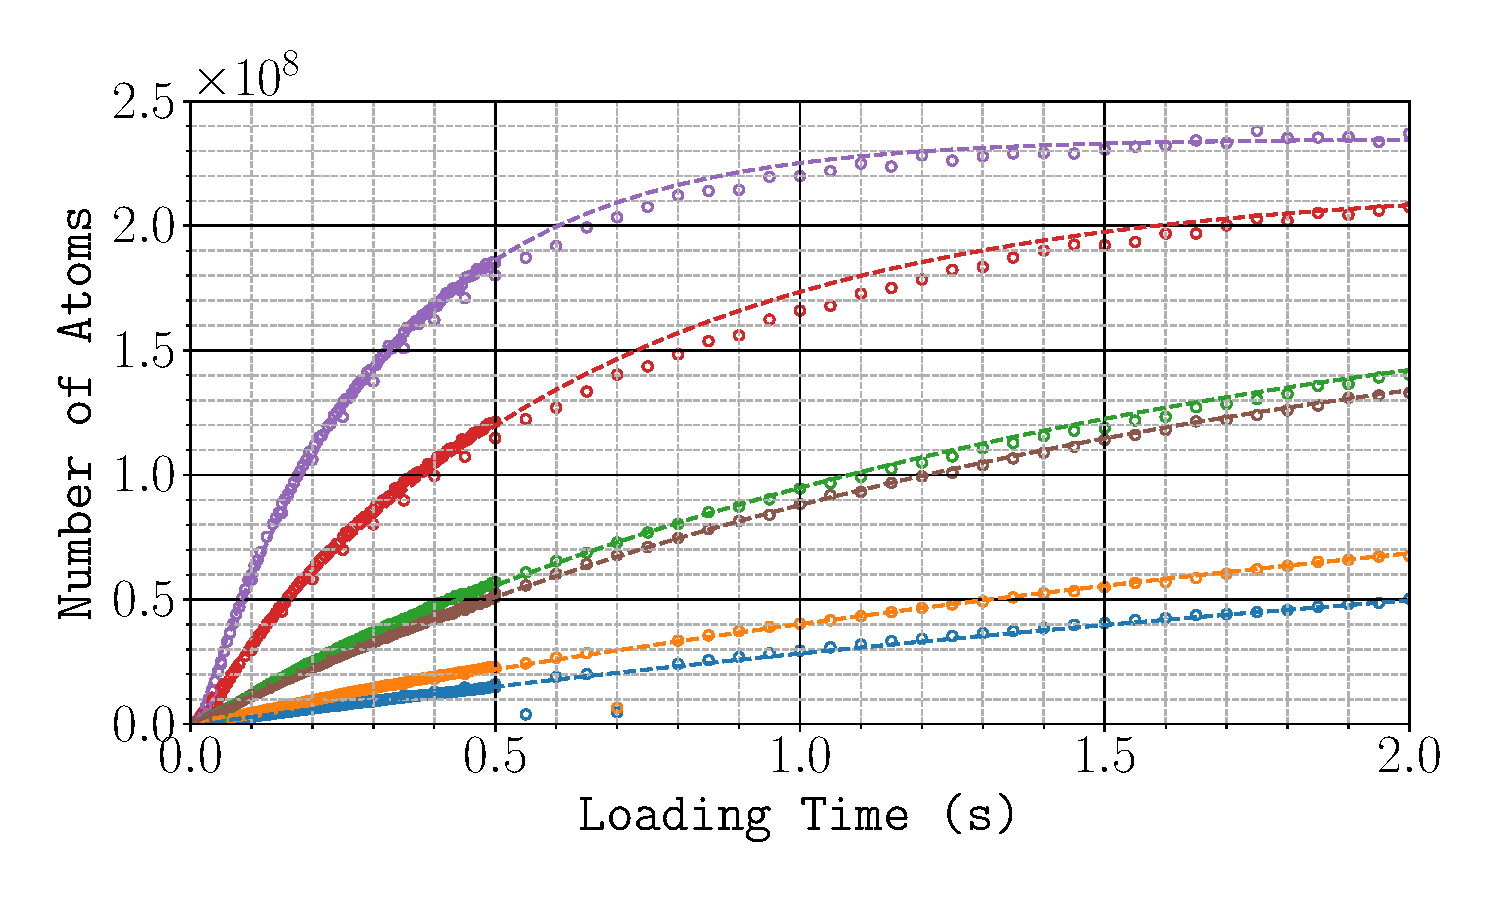
\includegraphics{Figures/Chapter4/loading_nopush.pdf}}\label{fig:loading_nopush}}
	\subfloat[][]{\scalebox{0.3}{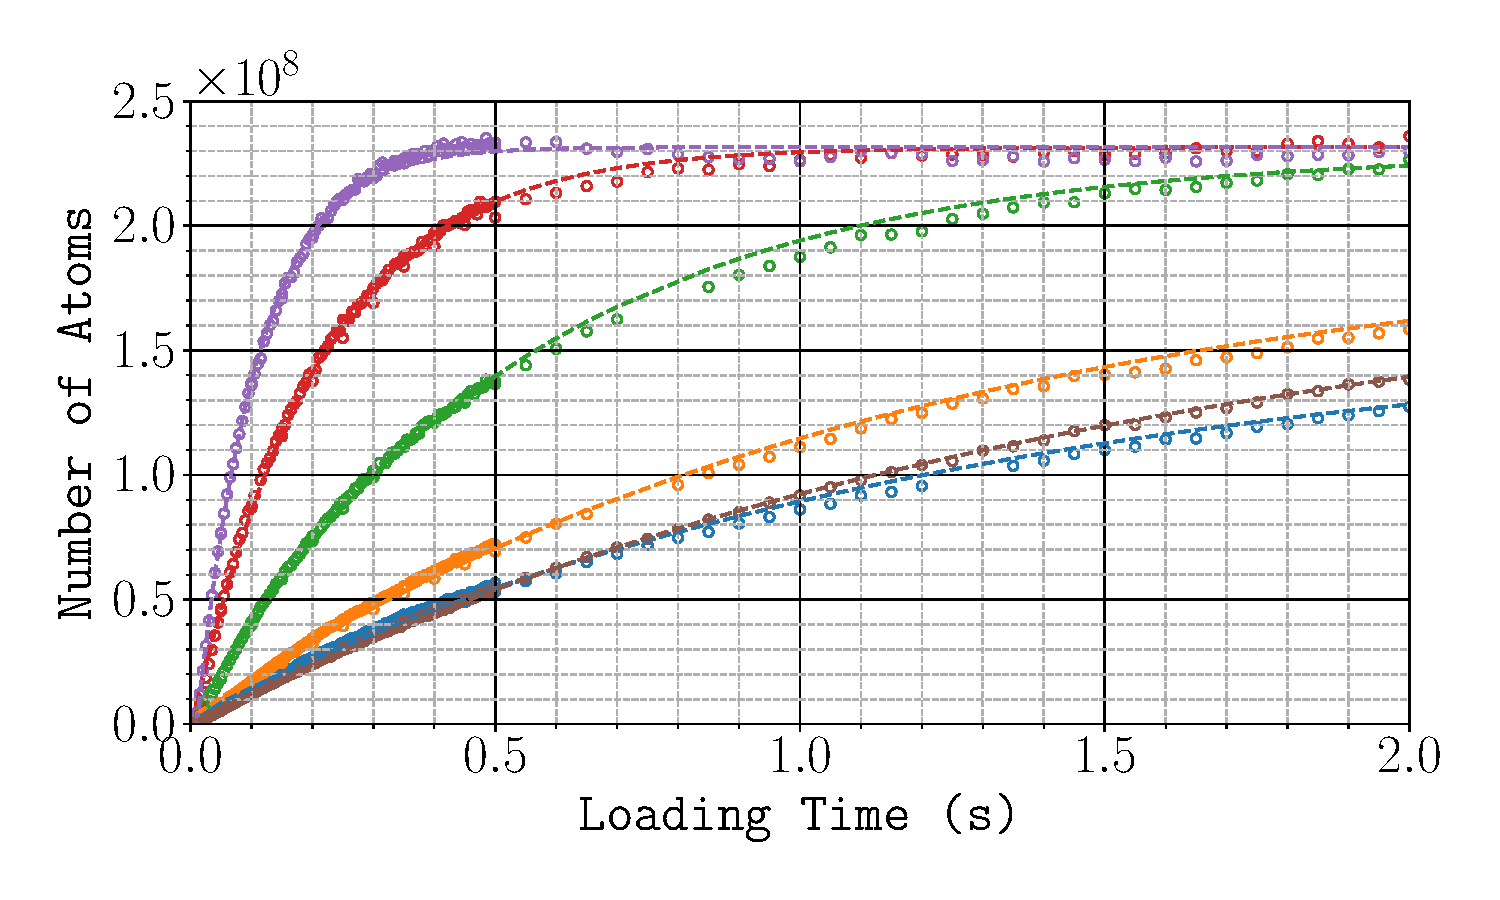
\includegraphics{Figures/Chapter4/loading_push.pdf}}\label{fig:loading_push}}\\
	\subfloat[][]{\scalebox{0.3}{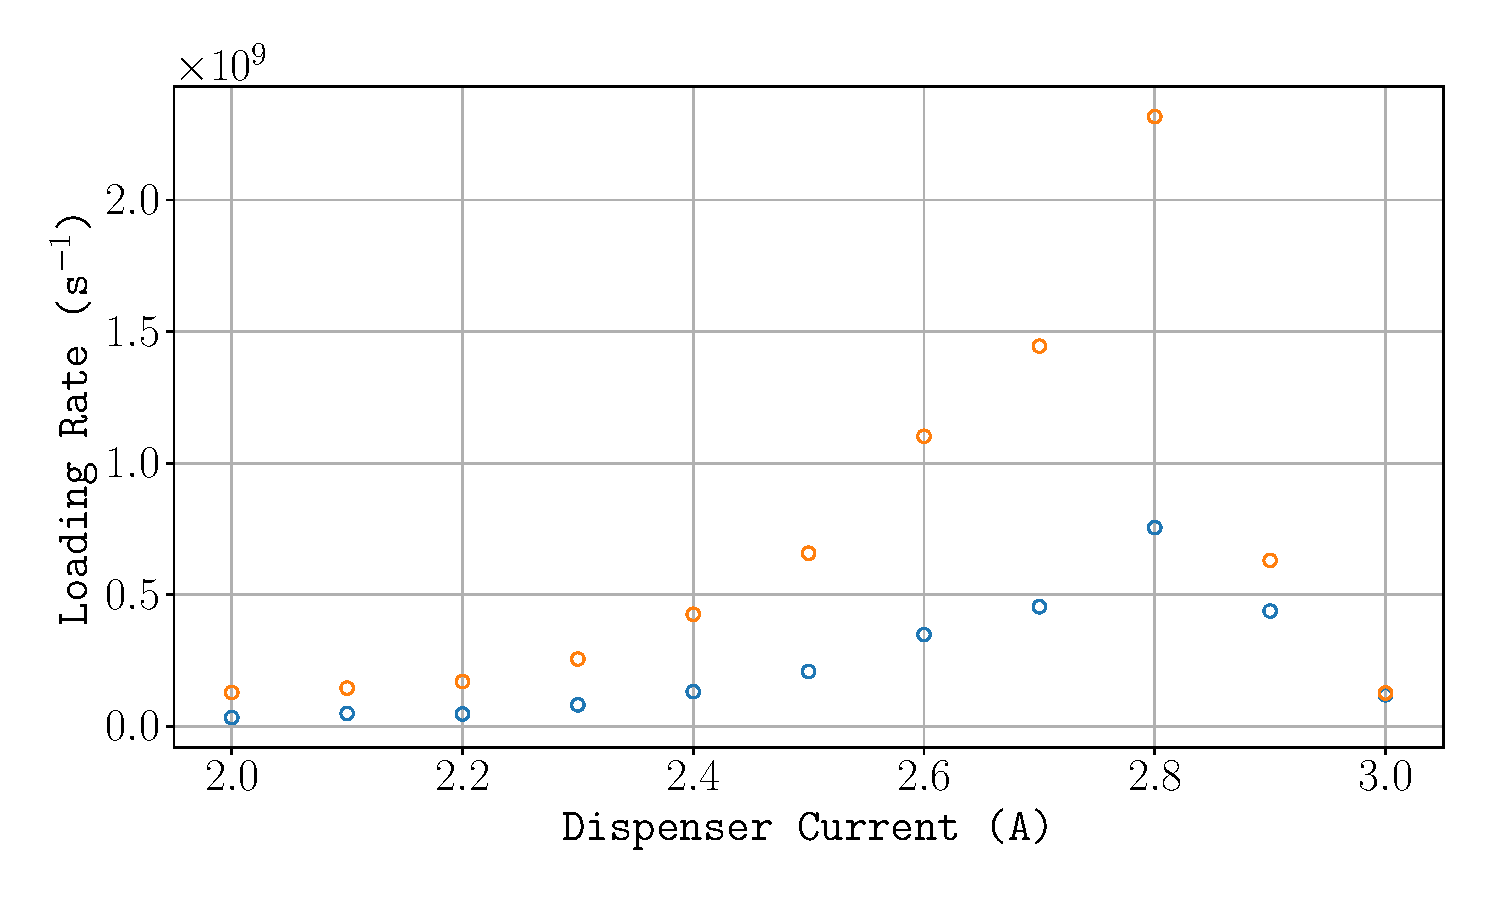
\includegraphics{Figures/Chapter4/loading_rate.pdf}}\label{fig:loading_rate}}
	\caption[3D \ac{mot} atom number vs dispenser current with and without a
		push beam.]{Number of atoms and loading rate for the 3D \ac{mot}
      $\textbf{(a)}$ without push beam and $\textbf{(b)}$ with push beam. For clarity, only the loading curves for dispenser
		currents of
		\sivalue{2}{\ampere} (blue),\sivalue{2.2}{\ampere}
		(orange), \sivalue{2.4}{\ampere} (green), \sivalue{2.6}{\ampere} (red),
		\sivalue{2.8}{\ampere} (purple) and \sivalue{3}{\ampere} (brown)
    $\textbf{(c)}$ Loading rates (\(R
    \phi_\text{rb}\) with (orange) and without (blue) push beam. 
		As the partial pressure of rubidium increases, the
		flux of atoms from the source cell increases. By longitudinally cooling
		the atoms, the push beam enhances the loading rate of the 3D \ac{mot}.
		Above a dispenser current of
		\sivalue{2.8}{\ampere}, the collision rate with hot untrapped atoms greatly reduces the atom flux, reducing both the loading rate and steady-state atom number.}
	\label{fig:loading_plots}
\end{figure}

\section{Conclusion}
This chapter has introduced the components of the experiment that were used to
trap and cool atoms in a \ac{mot}. This is used to prepare an ensemble of cold
atoms in a pure quantum state, suitable for interferometry. An optimisation of
the loading rate of the 3D \ac{mot} was carried out to reduce the dead time
between consecutive experiment cycles. 
